\documentclass[t]{beamer}

% --- Theme and Color Setup ---
\usetheme{Madrid}

\definecolor{MyBlue}{RGB}{0, 124, 193}

\usecolortheme[named=MyBlue]{structure}
\setbeamercolor{palette primary}{bg=MyBlue,fg=white}
\setbeamercolor{palette secondary}{bg=MyBlue!80!black,fg=white}
\setbeamercolor{palette tertiary}{bg=MyBlue!60!black,fg=white}
\setbeamerfont{caption}{size=\footnotesize}

% Packages
\usepackage[utf8]{inputenc}
\usepackage[spanish]{babel}
\usepackage{hyperref}
\usepackage{tikz}
\usepackage{booktabs}
\usepackage{graphicx}
\usepackage{amsmath}
\usepackage{colortbl}

\usetikzlibrary{arrows.meta, shapes.geometric, positioning}

% --- 1. CONFIGURATION FOR CONTENT SLIDES (Middle Pages) ---
\addtobeamertemplate{frametitle}{}{%
    \begin{tikzpicture}[remember picture,overlay]
        %\node[anchor=north east, xshift=-0.3cm, yshift=0cm, inner sep=0pt] at (current page.north east) {
        %    
\includegraphics[height=1cm, keepaspectratio]{imagenes/logo-fiblletres-upc-color.png}
        %};
    \end{tikzpicture}
}

% --- 2. CONFIGURATION FOR FIRST & LAST PAGE ---
\newcommand{\FirstLastPageLayout}{
    \begin{tikzpicture}[remember picture,overlay]
        \node[anchor=north, xshift=0cm, yshift=-0.3cm, inner sep=0pt] at (current page.north) {
            \begin{minipage}{0.10\paperwidth}
                \centering
                
\includegraphics[width=\textwidth]{imagenes/Logo_UPC.svg.png}
            \end{minipage}
            \hspace{0.02\paperwidth}
            \begin{minipage}{0.60\paperwidth}
                \centering
                
\includegraphics[width=\textwidth]{imagenes/logo-fiblletres-upc-color.png}
            \end{minipage}
        };
        %\node[anchor=south west, xshift=0.5cm, yshift=0.5cm] at (current page.south west) {
        %    \textcolor{MyBlue}{\footnotesize Facultat d'Informàtica de Barcelona -- UPC}
        %};
    \end{tikzpicture}
}

% --- Info ---

\title[Trabajo de Fin de Grado]{Sistema Inteligente de Asistencia al Desarrollo Estructurado y Seguimiento de Proyectos de software}
\author{Adrià Cebrián Ruiz}
\institute[FIB -- UPC]{Facultat d'Informàtica de Barcelona -- UPC}
\date{30/06/2026}

\begin{document}

% ============================================================
% SLIDE 1: TITLE PAGE
% ============================================================
\begin{frame}
    \FirstLastPageLayout
    \vspace{1cm}
    \titlepage
\end{frame}

% ============================================================
% SLIDE 2: ÍNDICE
% ============================================================
\begin{frame}{Índice}
    \begin{itemize}
        \item El problema a resolver
        \item Propuesta conceptual
        \item Estado del arte
        \item Diseño e implementación
        \item Experimentos y resultados
        \item Conclusiones
    \end{itemize}
\end{frame}

% ============================================================
% SLIDE 3: EL PROBLEMA A RESOLVER
% ============================================================
\begin{frame}{El problema a resolver}
    \begin{columns}[T]
        \begin{column}{0.38\textwidth}
            \vspace{0.3cm}
            El uso impulsivo de asistentes de IA genera un \textbf{ciclo vicioso} que degrada la calidad del código:
            \vspace{0.5cm}
            \begin{itemize}
                \item Prompt impulsivo
                \item Código sin estructura
                \item Bugs
                \item Parche rápido
                \item Deuda técnica
            \end{itemize}
        \end{column}
        \begin{column}{0.58\textwidth}
            \centering
            \vspace{0.2cm}
            \begin{tikzpicture}[
                node distance=0.8cm and 0.9cm,
                box/.style={rectangle, draw=MyBlue, fill=MyBlue, text=white,
                            minimum width=2.1cm, minimum height=0.75cm,
                            font=\small, align=center, rounded corners=2pt},
                arr/.style={-{Stealth[length=5pt]}, gray!70, line width=2.5pt, rounded corners=5pt}
            ]
                \node[box] (prompt) {Prompt\\impulsivo};
                \node[box, below right=of prompt] (codigo) {Código sin\\estructura};
                \node[box, below left=of codigo] (bugs) {Bugs};
                \node[box, left=1.5cm of bugs] (parche) {Parche\\rápido};
                \node[box, above left=of parche] (deuda) {Deuda\\técnica};

                \draw[arr] (deuda.north) -- ++(0,0.6) -| (prompt.west);
                \draw[arr] (prompt.east) -- ++(0.5,0) |- (codigo.north);
                \draw[arr] (codigo.south) -- ++(0,-0.3) -| (bugs.east);
                \draw[arr] (bugs.west) -- (parche.east);
                \draw[arr] (parche.north) -- (deuda.south);
            \end{tikzpicture}
        \end{column}
    \end{columns}
\end{frame}

% ============================================================
% SLIDE 4: PROPUESTA CONCEPTUAL
% ============================================================
\begin{frame}{Propuesta conceptual}
    \begin{columns}[T]
        \begin{column}{0.40\textwidth}
            \textbf{Tres pilares principales:}
            \begin{itemize}
                \item Toma de requerimientos
                \item Spec-Driven Development
                \item Seguimiento del cliente
            \end{itemize}
            \vspace{0.4cm}
            Construidos basándonos en los siguientes principios:
            \begin{itemize}
                \item \textit{Human-in-the-loop}
                \item Documentación estructurada
                \item Compatibilidad con asistentes existentes
            \end{itemize}
        \end{column}
        \begin{column}{0.57\textwidth}
            \begin{figure}
                
\includegraphics[width=\linewidth, keepaspectratio]{imagenes/DiagramaFlujoTrabajoCompleto.png}
            \end{figure}
        \end{column}
    \end{columns}
\end{frame}

% ============================================================
% SLIDE 5: ESTADO DEL ARTE – DESARROLLO DE CÓDIGO
% ============================================================
\begin{frame}{Estado del arte -- Desarrollo de código}
    Asistentes comerciales, \textbf{code-driven} de forma predeterminada:
    \vspace{0.4cm}

    \begin{columns}[c]
        \begin{column}{0.33\textwidth}
            \centering
            \texttt{\textbf{ClaudeCode}}
        \end{column}
        \begin{column}{0.33\textwidth}
            \centering
            \texttt{\textbf{Copilot}}
        \end{column}
        \begin{column}{0.33\textwidth}
            \centering
            \texttt{\textbf{OpenCode}}
        \end{column}
    \end{columns}

    \vspace{0.5cm}
    Soluciones \textbf{spec-first}, construidas para expandir estos asistentes:
    \vspace{0.3cm}

    \begin{columns}[T]
        \begin{column}{0.33\textwidth}
            \footnotesize
            \textbf{obra/superpowers}\\
            An agentic skills framework \& software development methodology.
        \end{column}
        \begin{column}{0.33\textwidth}
            \footnotesize
            \textbf{GitHub Spec Kit}\\
            Define what to build before building it -- with any AI coding agent.
        \end{column}
        \begin{column}{0.33\textwidth}
            \footnotesize
            \textbf{Agent OS}\\
            Agents that build the way you would.
        \end{column}
    \end{columns}
\end{frame}

% ============================================================
% SLIDE 6: ESTADO DEL ARTE – PARTE 2
% ============================================================
\begin{frame}{Estado del arte -- Parte 2}
    \begin{columns}[T]
        \begin{column}{0.50\textwidth}
            \textbf{Documentación de reuniones:}
            \vspace{0.4cm}
            \begin{itemize}
                \item Otter.ai
                \item Fireflies.ai
            \end{itemize}
        \end{column}
        \begin{column}{0.47\textwidth}
            \textbf{Claude Cowork:}
            \vspace{0.3cm}
            \begin{figure}
                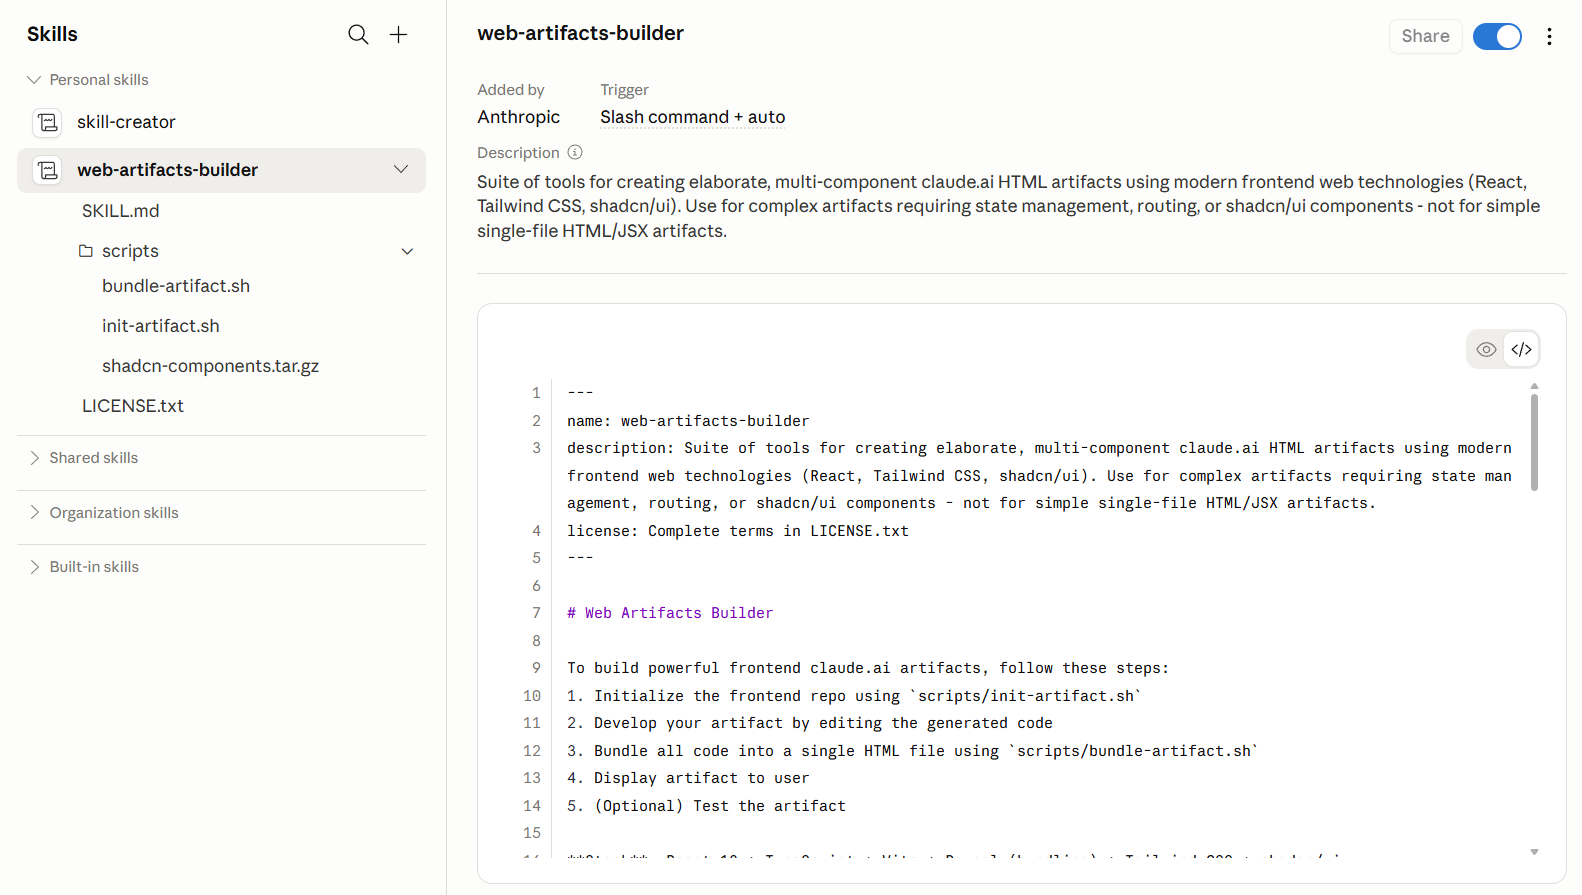
\includegraphics[width=\linewidth, keepaspectratio]{imagenes/coworkSkills/skill_components_and_definition.png}
            \end{figure}
        \end{column}
    \end{columns}
\end{frame}

% ============================================================
% SLIDE 7: DISEÑO SIMPLIFICADO DE LA IMPLEMENTACIÓN
% ============================================================
\begin{frame}{Diseño simplificado de la implementación}
    \begin{figure}
        \centering
        
\includegraphics[width=0.92\linewidth, keepaspectratio]{imagenes/DiagramaFlujoTrabajoCompleto.png}
    \end{figure}
\end{frame}

% ============================================================
% SLIDE 8: DIFERENCIA DISEÑO Y ESTADO DEL ARTE
% ============================================================
\begin{frame}{Diferencia diseño y estado del arte}
    \begin{itemize}
        \item \textbf{Integración completa:} el sistema engloba toma de requerimientos, desarrollo y seguimiento en un único flujo coherente.
        \vspace{0.3cm}
        \item \textbf{Spec-Driven por defecto:} la IA no genera código sin una especificación previa aprobada por el usuario.
        \vspace{0.3cm}
        \item \textbf{Human-in-the-loop:} el usuario valida en cada etapa crítica (plan, especificación, implementación).
        \vspace{0.3cm}
        \item \textbf{Compatible} con asistentes existentes (ClaudeCode, Opencode) sin modificarlos.
    \end{itemize}
\end{frame}

% ============================================================
% SLIDE 9: SOSTENIBILIDAD
% ============================================================
\begin{frame}{Sostenibilidad}
    \begin{columns}[T]
        \begin{column}{0.32\textwidth}
            \centering\textbf{Económica}
            \rule{\linewidth}{0.4pt}\\[0.2cm]
            \footnotesize
            Mayor inversión inicial, a cambio de un código mejor documentado. Reduce el tiempo que otros desarrolladores deben invertir en entender el código.\\[0.3cm]
            La metodología fomenta la creación de tests de prueba, ahorrando costes de mantenimiento.
        \end{column}
        \begin{column}{0.32\textwidth}
            \centering\textbf{Ambiental}
            \rule{\linewidth}{0.4pt}\\[0.2cm]
            \footnotesize
            Consumo inicial elevado, pero mejor documentado. La metodología SDD genera documentación que reduce el uso posterior de IA.\\[0.3cm]
            Los tests de prueba reducen la cantidad de \textit{prompts} para solucionar errores inesperados.
        \end{column}
        \begin{column}{0.32\textwidth}
            \centering\textbf{Social}
            \rule{\linewidth}{0.4pt}\\[0.2cm]
            \footnotesize
            La metodología Human-in-the-loop conlleva mayor involucra\-miento del desarrollador como profesional.\\[0.3cm]
            La generación de documentación facilita la incorporación de talento nuevo en los proyectos.
        \end{column}
    \end{columns}
\end{frame}

% ============================================================
% SLIDE 10: SECTION DIVIDER – IMPLEMENTACIÓN (no cuenta en el total)
% ============================================================
\begin{frame}[plain,noframenumbering]
\begin{tikzpicture}[remember picture, overlay]
    \fill[MyBlue] (current page.south west) rectangle (current page.north east);
\end{tikzpicture}
\vspace{0.38\textheight}
\begin{center}
    \textcolor{white}{\LARGE Implementación}
\end{center}
\end{frame}

% ============================================================
% SLIDE 11: TRANSCRIPCIÓN
% ============================================================
\begin{frame}{Transcripción}
    \begin{columns}[T]
        \begin{column}{0.40\textwidth}
            \vspace{0.3cm}
            Tecnologías utilizadas:
            \begin{itemize}
                \item \textbf{FFmpeg} -- compresión de audio y cálculo de hash
                \item \textbf{Azure Speech-to-Text} -- transcripción
                \item \textbf{Azure Blob Storage} -- caché de resultados
            \end{itemize}
            \vspace{0.3cm}
            El hash permite reutilizar transcripciones previas evitando llamadas repetidas a la API.
        \end{column}
        \begin{column}{0.57\textwidth}
            \begin{figure}
                
\includegraphics[width=\linewidth, keepaspectratio]{imagenes/Transcription System.png}
            \end{figure}
        \end{column}
    \end{columns}
\end{frame}

% ============================================================
% SLIDE 12: TOMA DE REQUERIMIENTOS – CLAUDECOWORK
% ============================================================
\begin{frame}{Toma de requerimientos -- ClaudeCowork}
    \begin{figure}
        \centering
        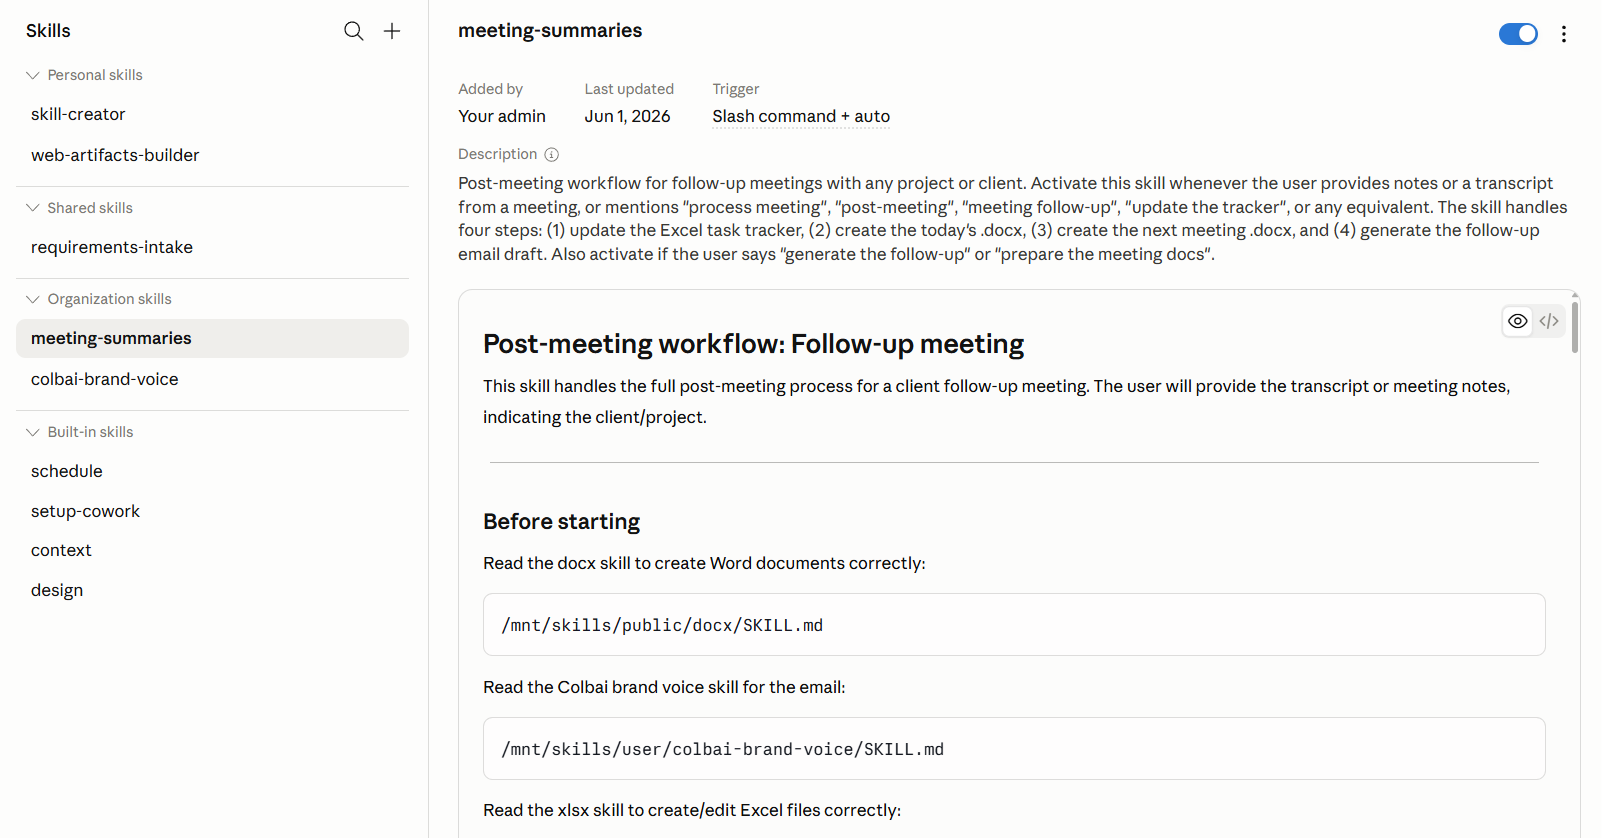
\includegraphics[width=0.88\linewidth, keepaspectratio]{imagenes/meeting_summaries_skill.png}
        \caption{Skill \texttt{meeting-summaries} en Claude Cowork}
    \end{figure}
\end{frame}

% ============================================================
% SLIDE 13: TOMA DE REQUERIMIENTOS – IMPLEMENTACIÓN PROPIA
% ============================================================
\begin{frame}{Toma de requerimientos -- Implementación propia}
    \begin{figure}
        \centering
        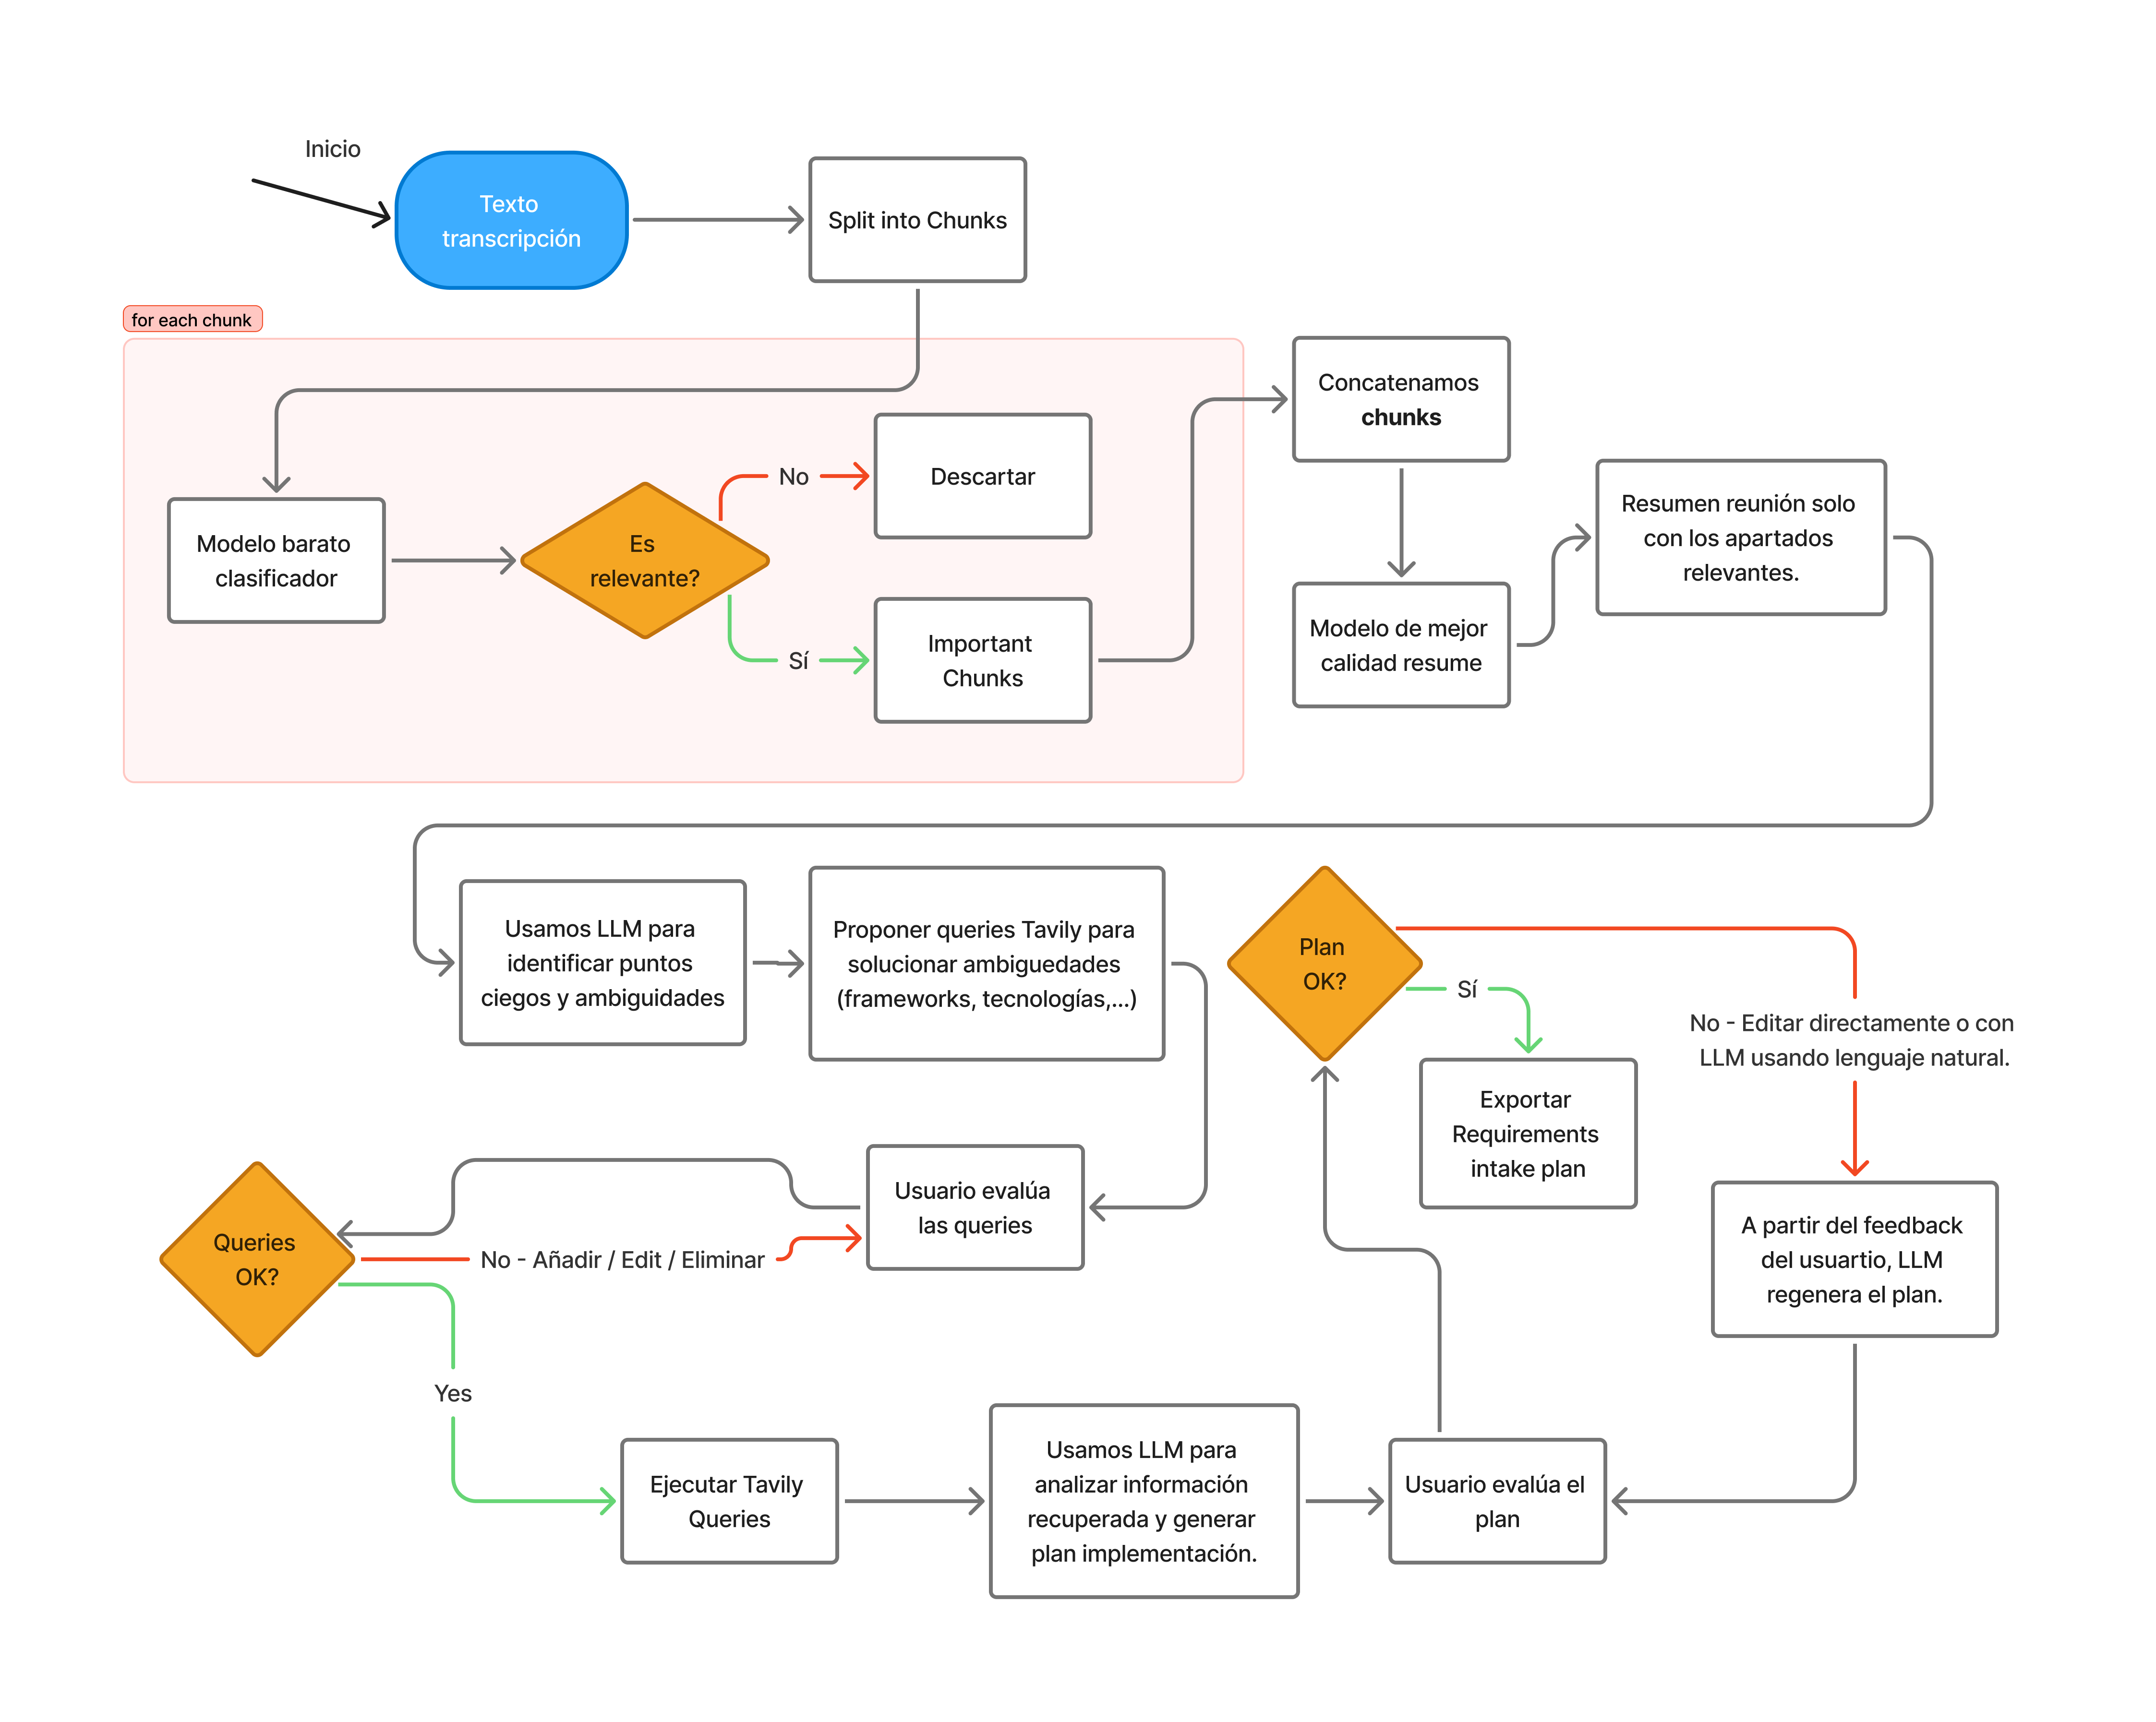
\includegraphics[width=0.88\linewidth, keepaspectratio]{imagenes/Requirements Intake System.png}
        \caption{Flujo del sistema de toma de requerimientos}
    \end{figure}
\end{frame}

% ============================================================
% SLIDE 14: SEGUIMIENTO DE CLIENTE – CLAUDECOWORK
% ============================================================
\begin{frame}{Seguimiento de cliente -- ClaudeCowork}
    \begin{figure}
        \centering
        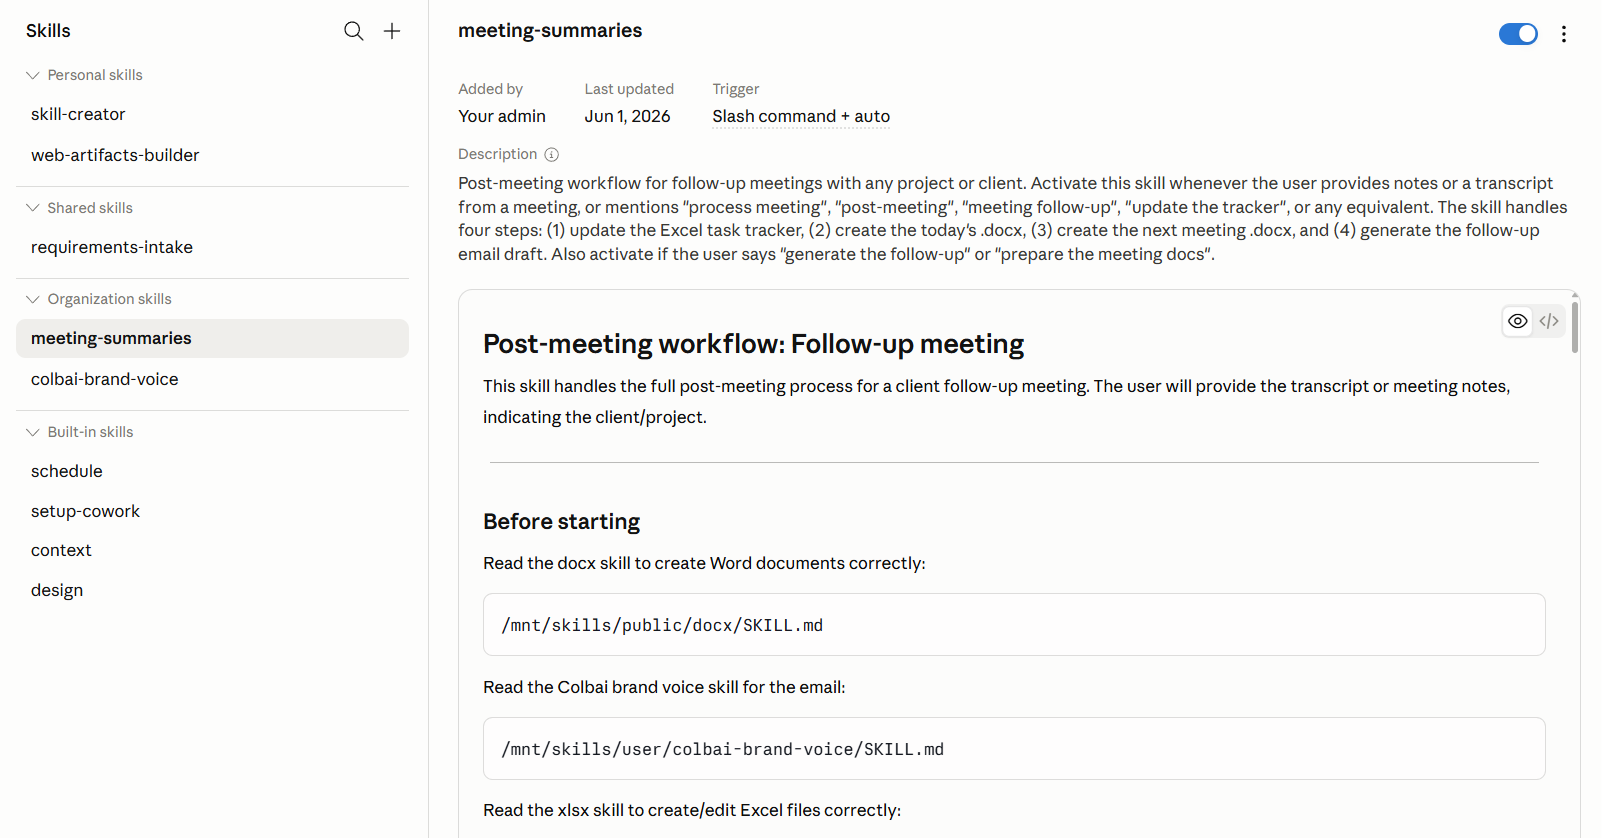
\includegraphics[width=0.88\linewidth, keepaspectratio]{imagenes/meeting_summaries_skill.png}
        \caption{Skill \texttt{meeting-summaries} en Claude Cowork}
    \end{figure}
\end{frame}

% ============================================================
% SLIDE 15: SEGUIMIENTO DE CLIENTE – IMPLEMENTACIÓN PROPIA
% ============================================================
\begin{frame}{Seguimiento de cliente -- Implementación propia}
    \begin{figure}
        \centering
        
\includegraphics[width=0.88\linewidth, keepaspectratio]{imagenes/SeguimientDelCliente.png}
        \caption{Flujo del sistema de seguimiento de cliente}
    \end{figure}
\end{frame}

% ============================================================
% SLIDE 16: SPEC-DRIVEN DEVELOPMENT – PART 1
% ============================================================
\begin{frame}{Spec-Driven Development -- Parte 1}
    \begin{columns}[T]
        \begin{column}{0.50\textwidth}
            Expansión de \textit{Superpowers} $\rightarrow$ \textbf{colbPowers}:
            \vspace{0.3cm}
            \begin{itemize}
                \item Adaptar skills existentes
                \item Añadir \texttt{constitution.md} + \texttt{features.md}
                \item Skills \textit{definingConstitution} y \textit{definingFeatures}
            \end{itemize}
            \vspace{0.4cm}
            \begin{figure}
                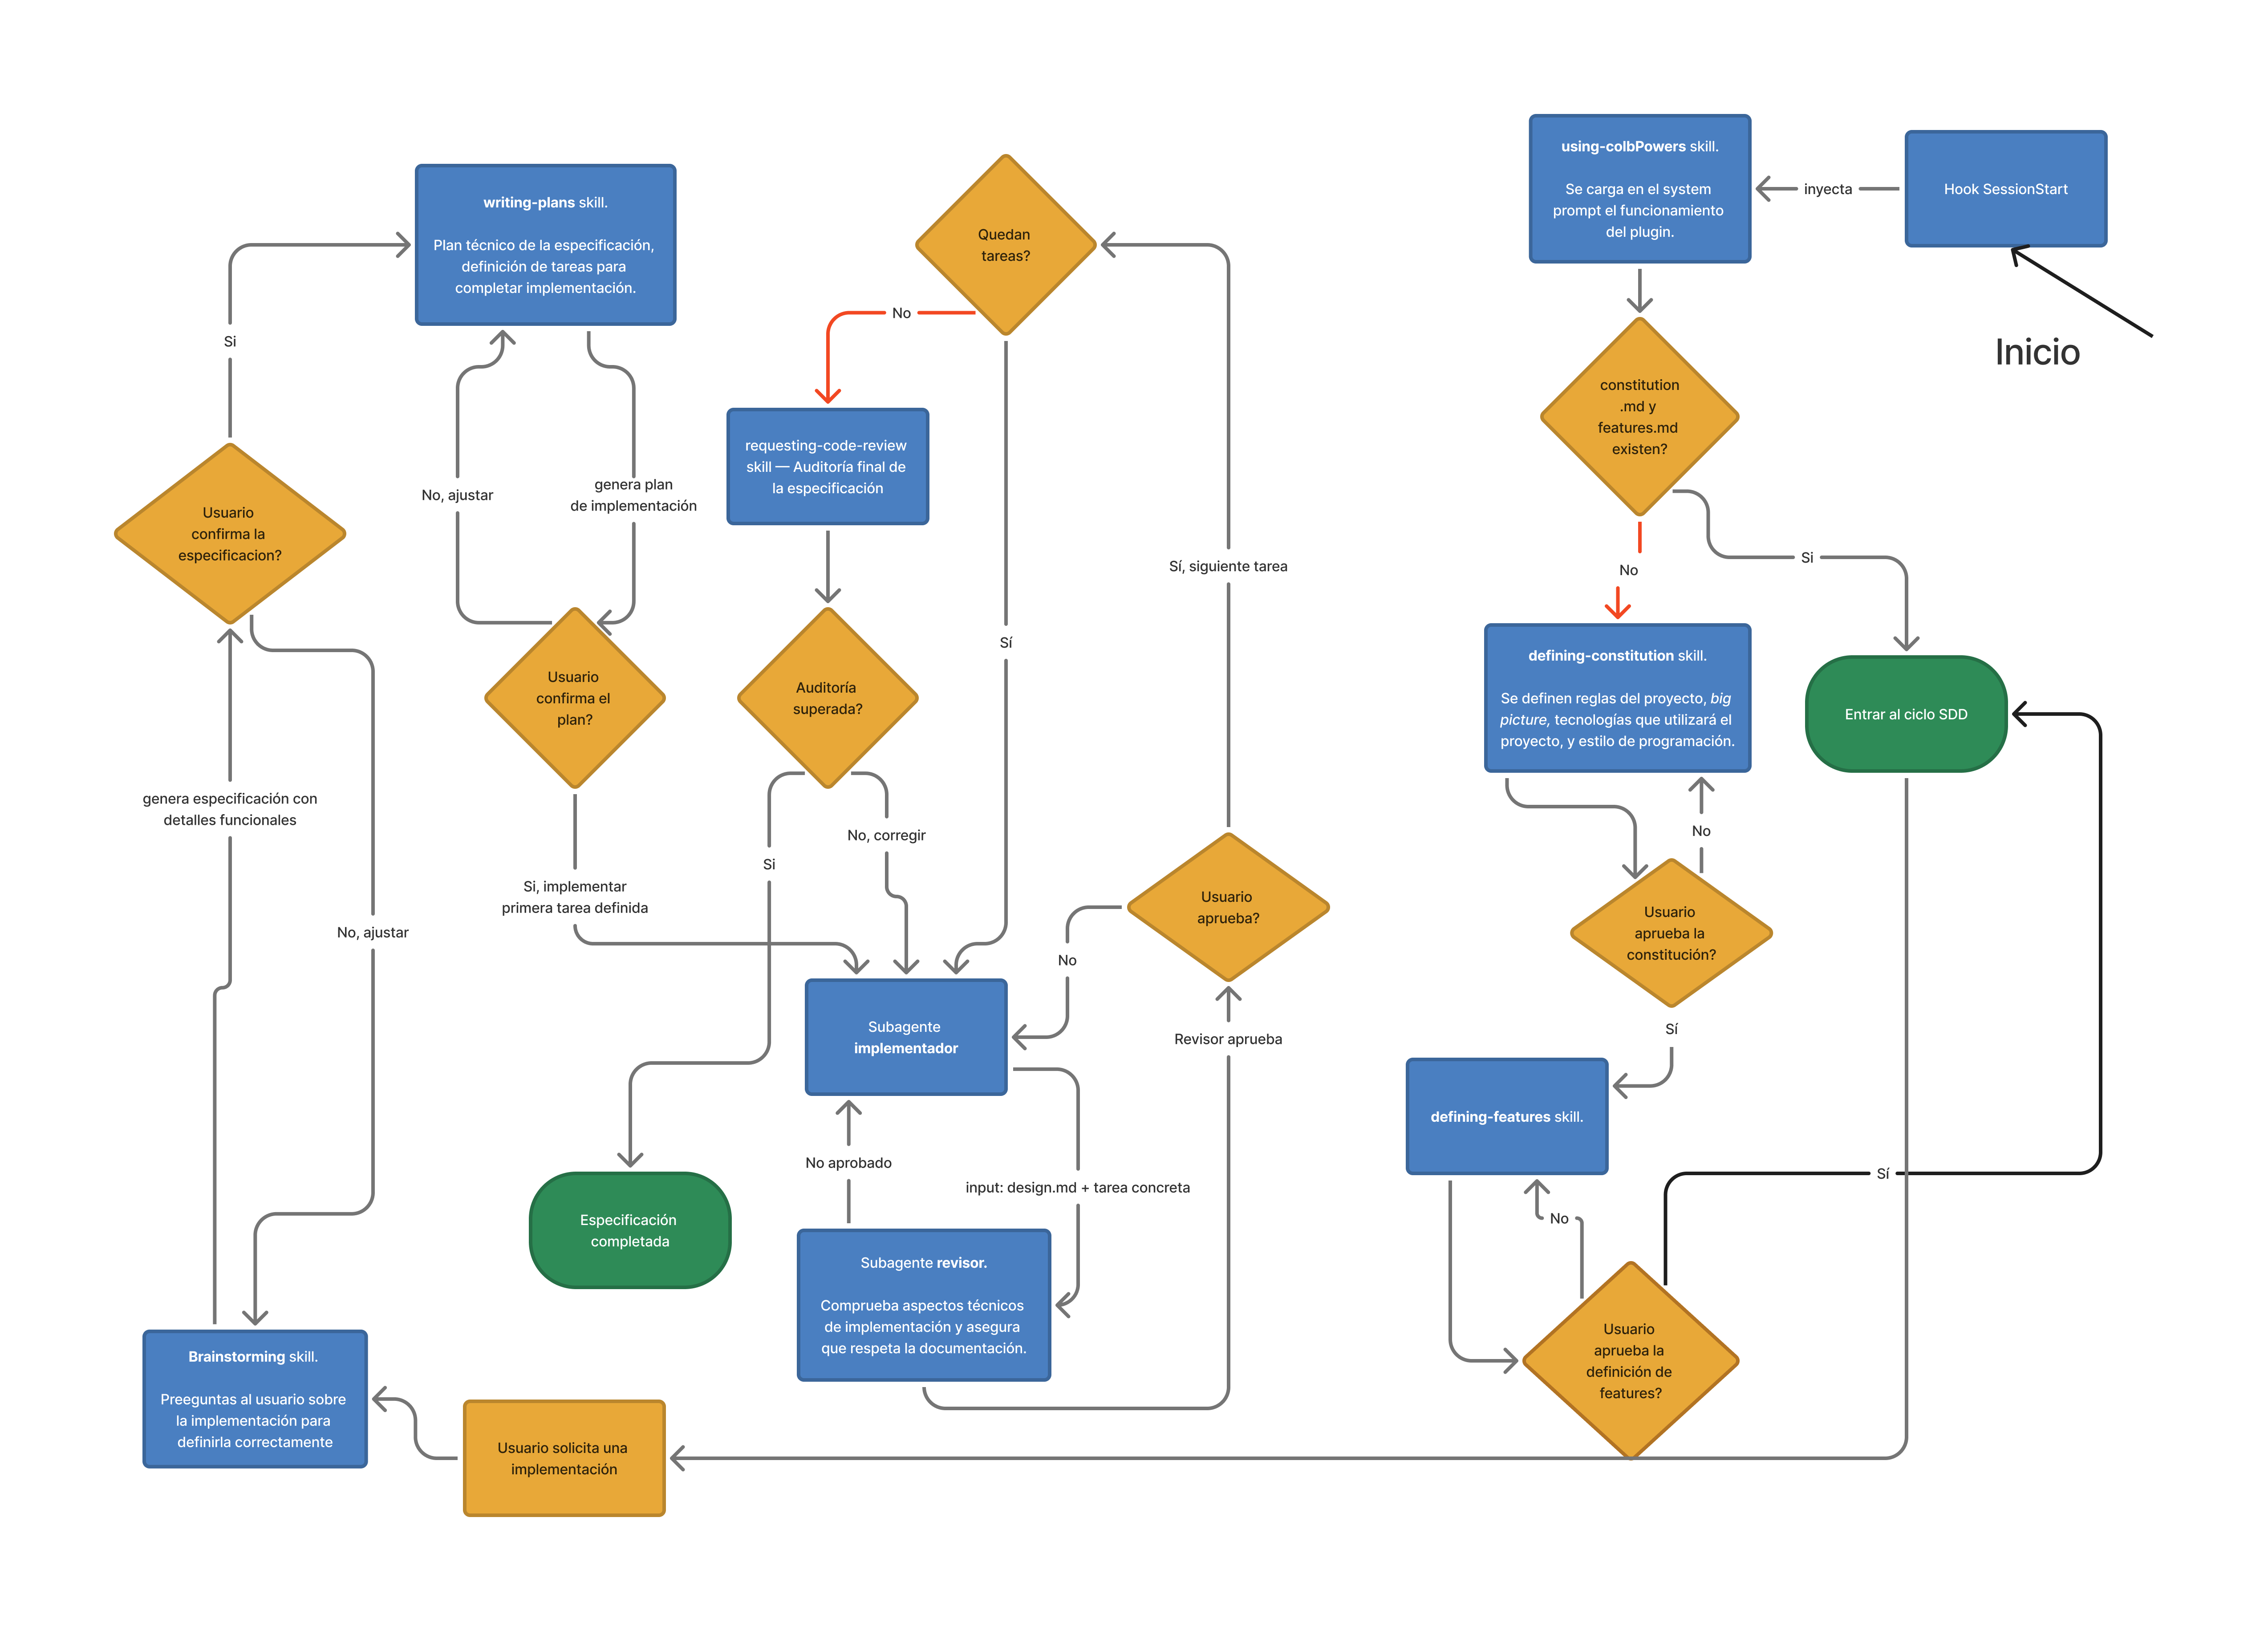
\includegraphics[width=0.9\linewidth, keepaspectratio]{imagenes/JustColbPowers.png}
            \end{figure}
        \end{column}
        \begin{column}{0.47\textwidth}
            Implementación compatible con \textbf{OpenCode} y \textbf{ClaudeCode}.
            \vspace{0.3cm}
            \begin{figure}
                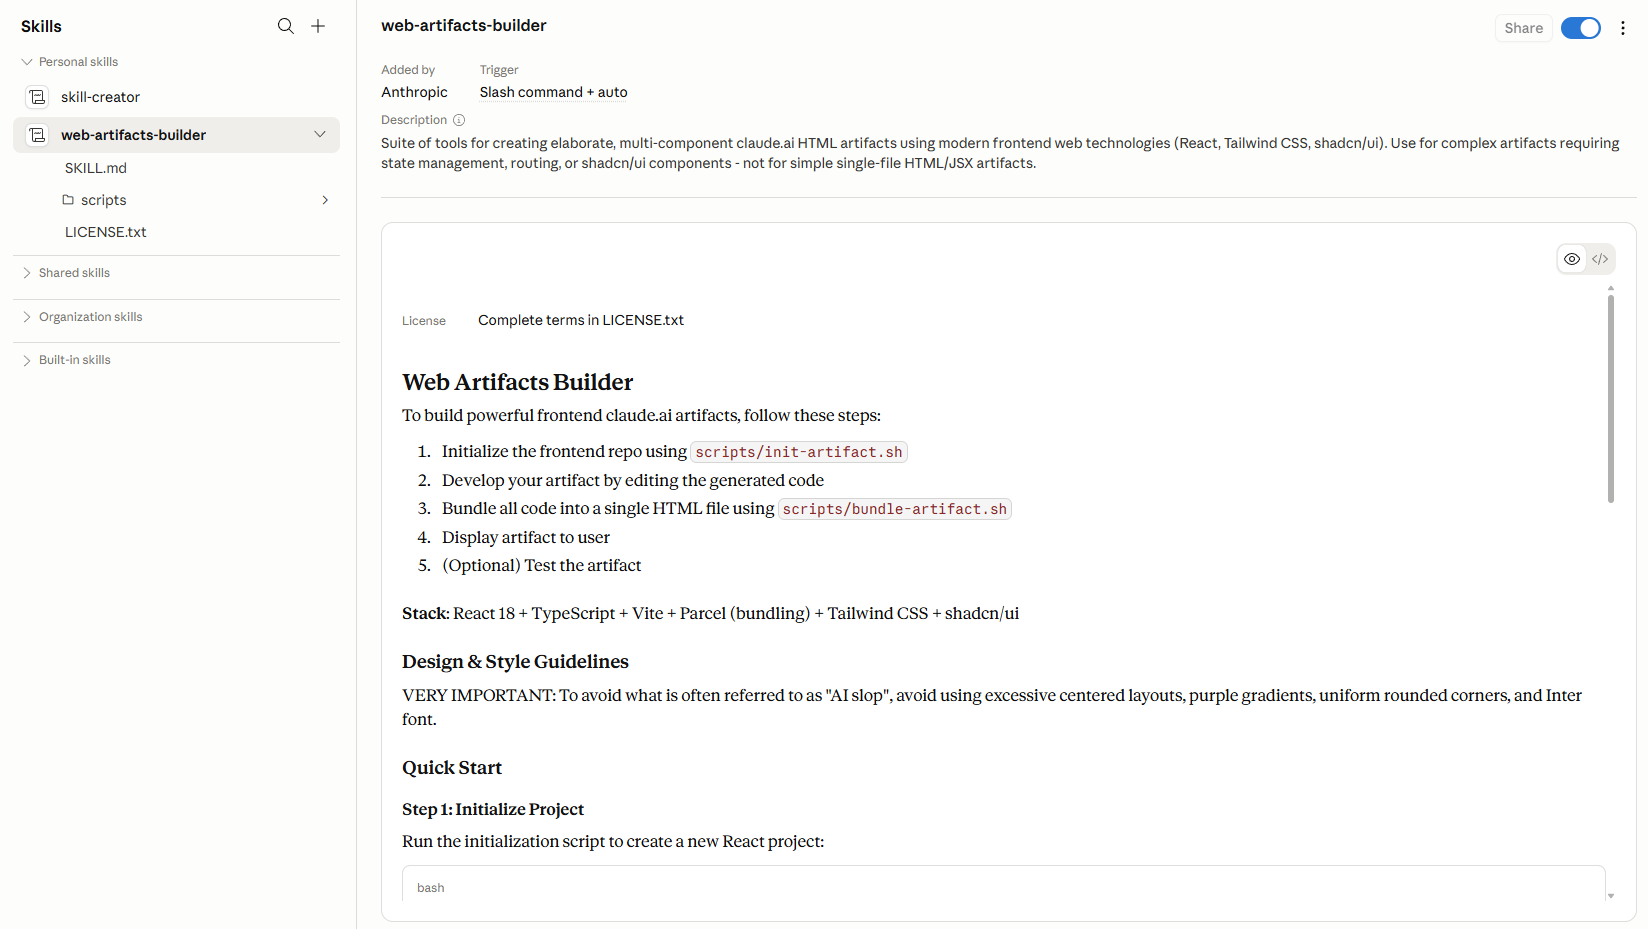
\includegraphics[width=\linewidth, keepaspectratio]{imagenes/coworkSkills/skill_components_and_definition2.png}
            \end{figure}
        \end{column}
    \end{columns}
\end{frame}

% ============================================================
% SLIDE 17: SPEC-DRIVEN DEVELOPMENT – PART 2
% ============================================================
\begin{frame}{Spec-Driven Development -- Parte 2}
    \begin{figure}
        \centering
        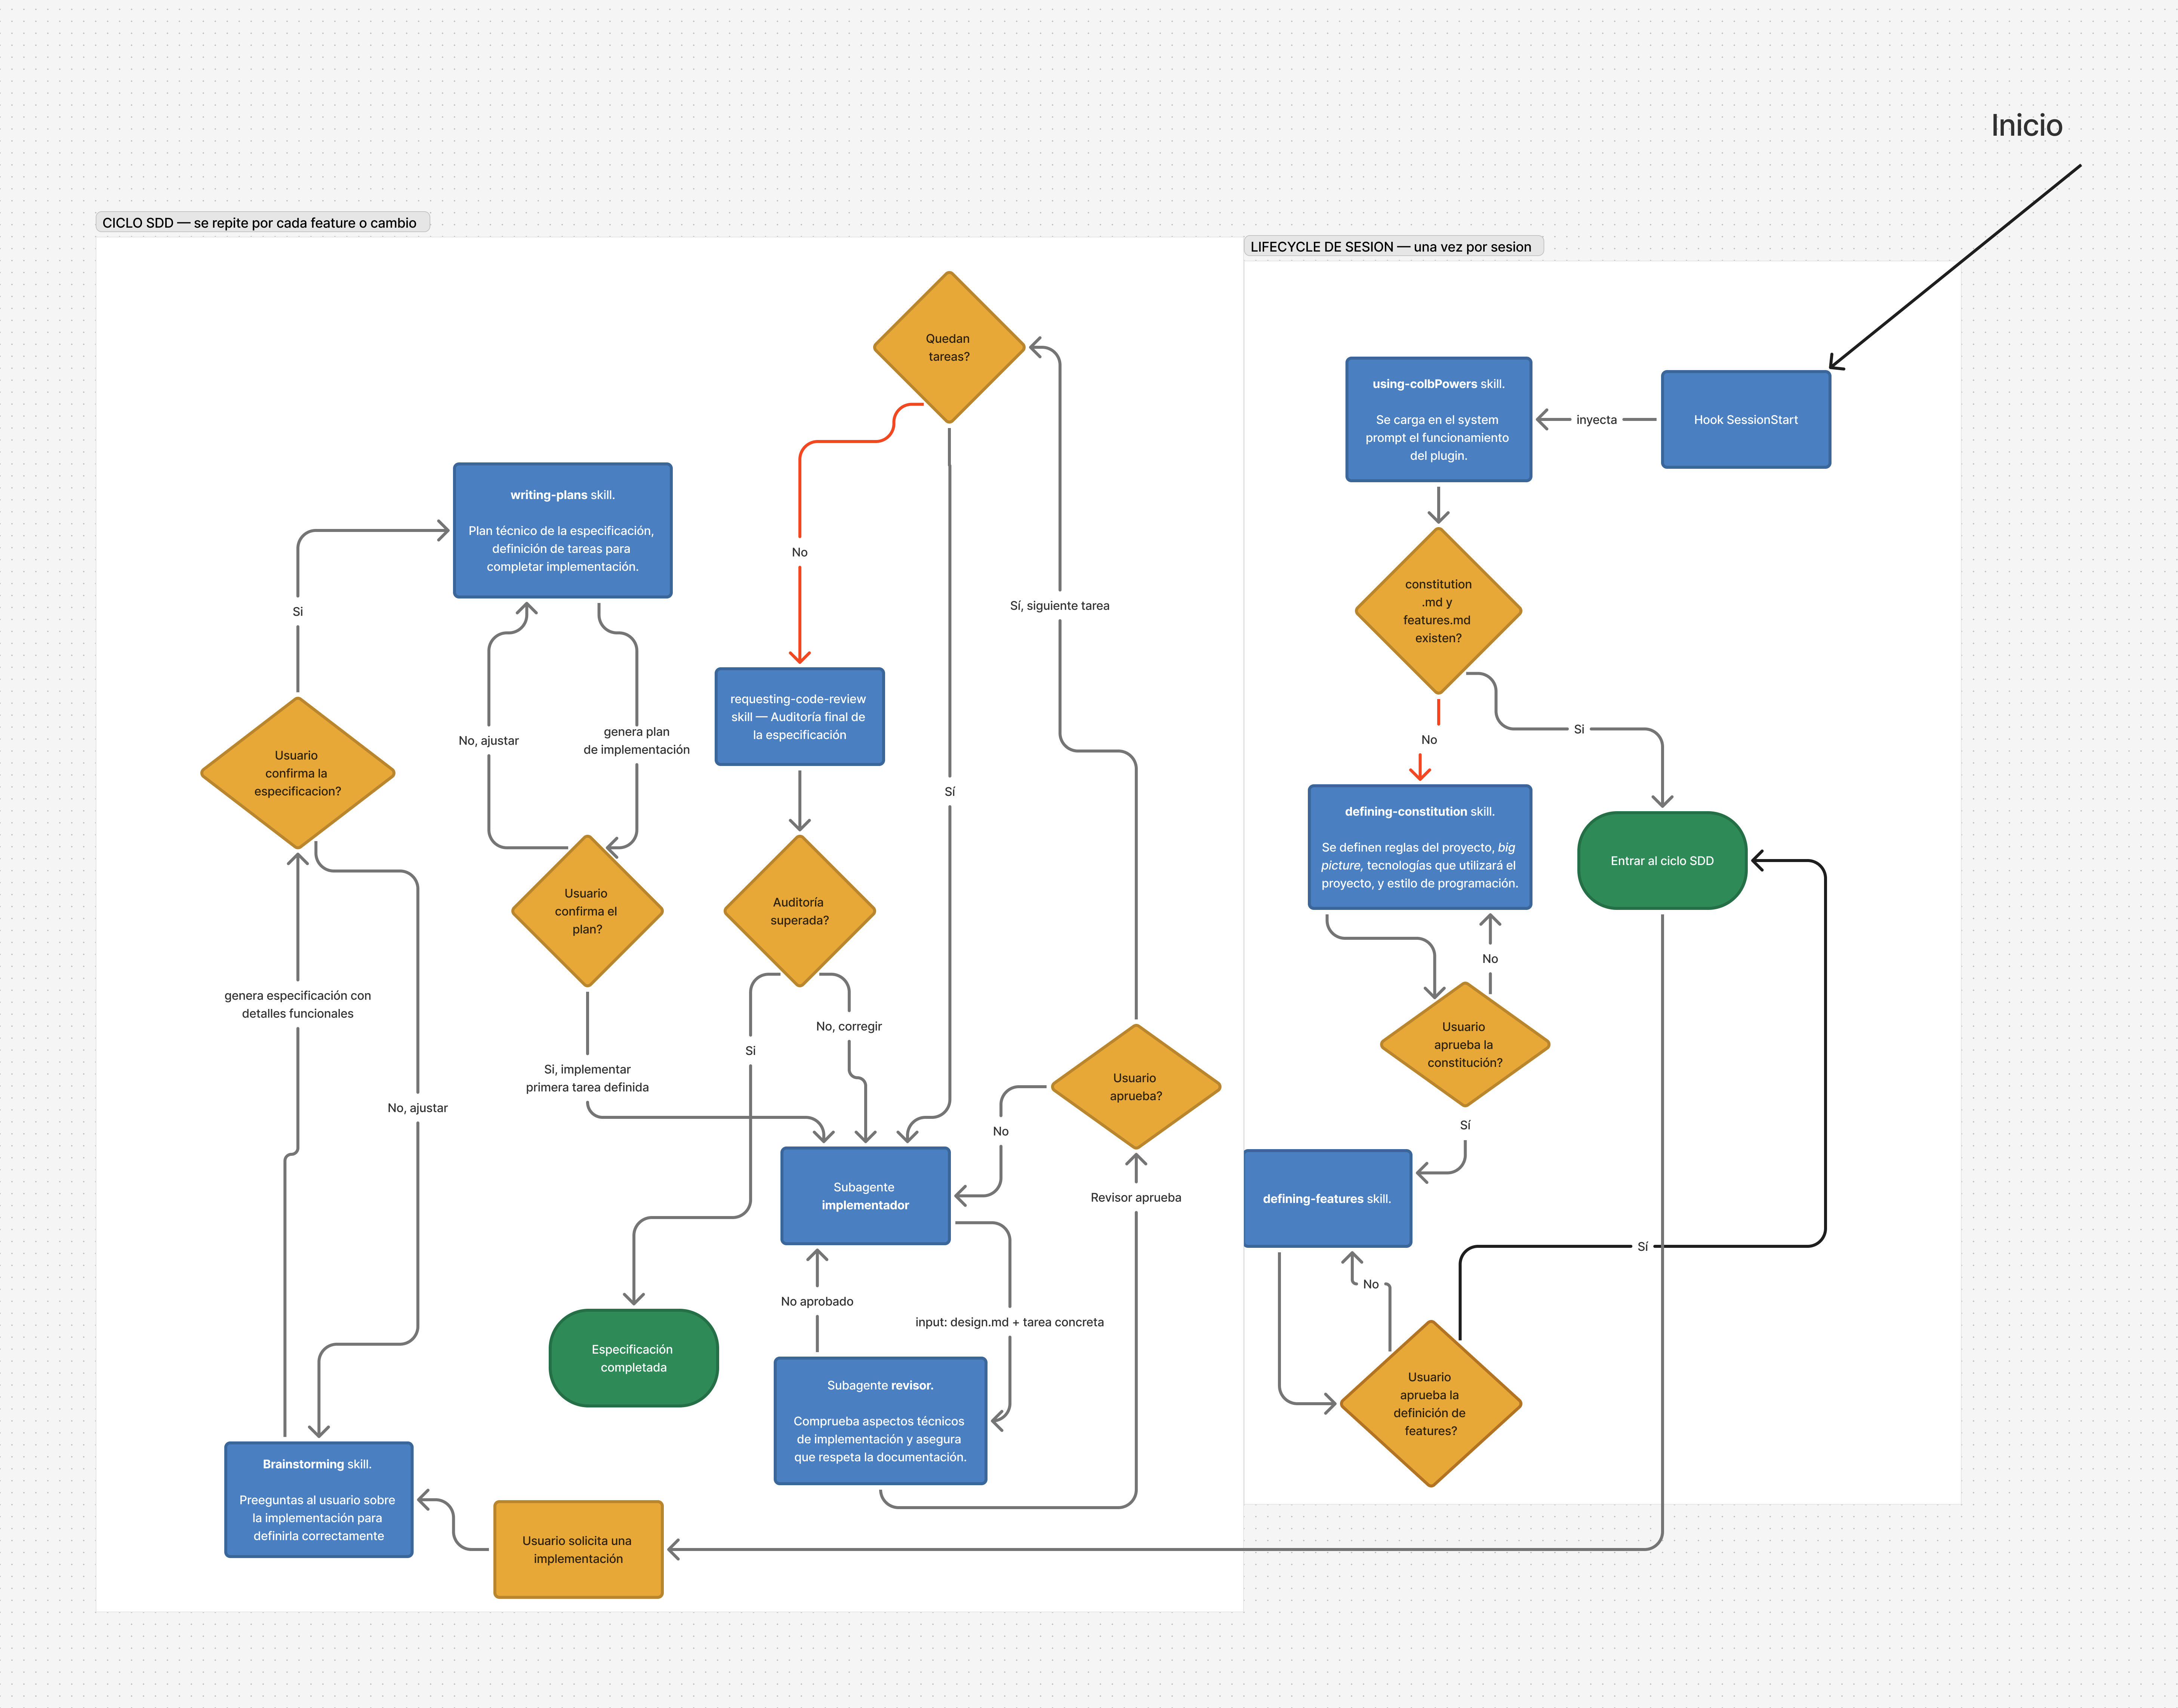
\includegraphics[width=0.92\linewidth, keepaspectratio]{imagenes/FlowColbPowers.png}
        \caption{Flujo completo de colbPowers}
    \end{figure}
\end{frame}

% ============================================================
% SLIDE 18: SPEC-DRIVEN DEVELOPMENT – PART 3
% ============================================================
\begin{frame}{Spec-Driven Development -- Parte 3}
    \begin{columns}[T]
        \begin{column}{0.62\textwidth}
            \begin{figure}
                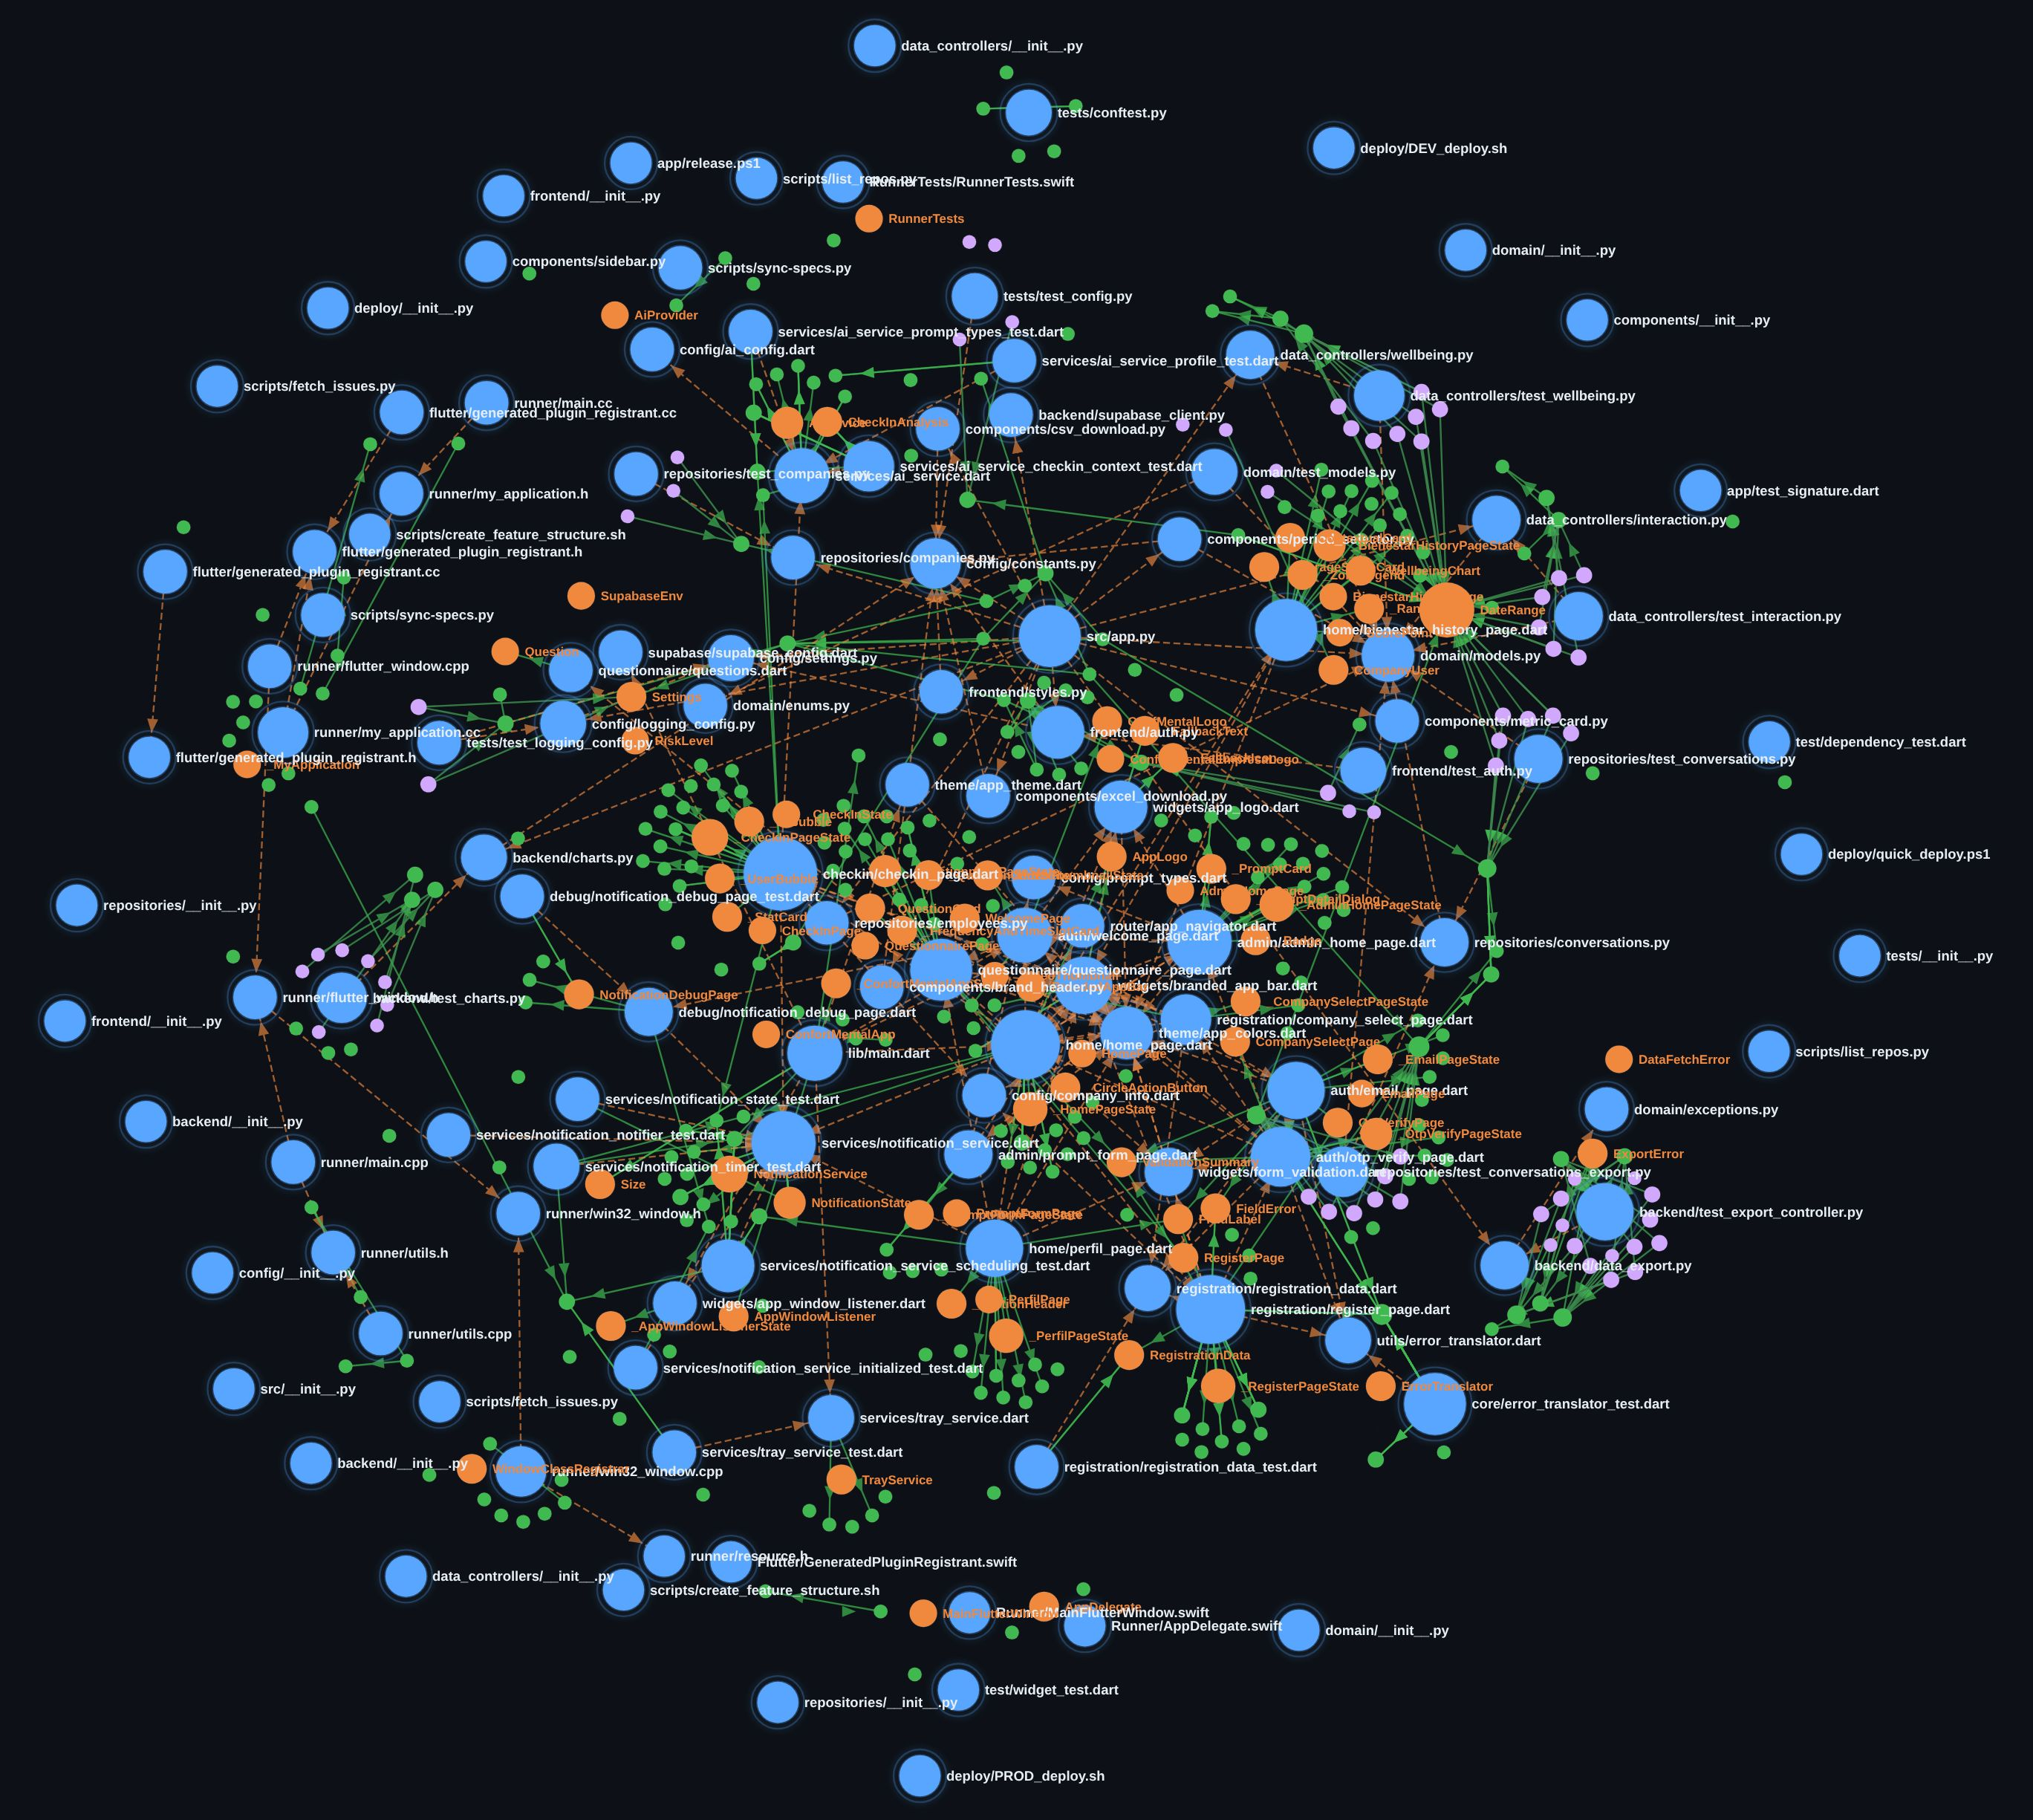
\includegraphics[width=\linewidth, keepaspectratio]{imagenes/code_review_graph_OnlyTheGraph.jpg}
            \end{figure}
        \end{column}
        \begin{column}{0.35\textwidth}
            \textbf{code-review-graph:}\\[0.3cm]
            Herramienta MCP para facilitar a los asistentes de programación la exploración del repositorio.
            \vspace{0.3cm}
            \begin{figure}
                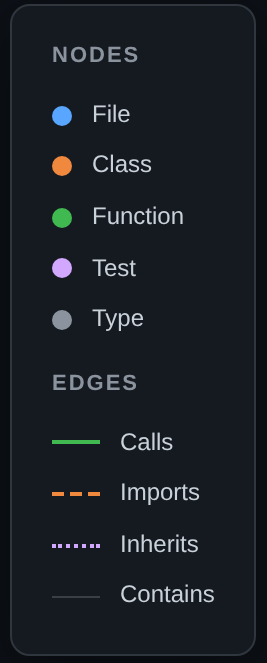
\includegraphics[width=\linewidth, keepaspectratio]{imagenes/code_review_graph_NodeTypes.png}
            \end{figure}
        \end{column}
    \end{columns}
\end{frame}

% ============================================================
% SLIDE 19: SECTION DIVIDER – EXPERIMENTOS
% ============================================================
\begin{frame}[plain,noframenumbering]
\begin{tikzpicture}[remember picture, overlay]
    \fill[MyBlue] (current page.south west) rectangle (current page.north east);
\end{tikzpicture}
\vspace{0.38\textheight}
\begin{center}
    \textcolor{white}{\LARGE Experimentos}
\end{center}
\end{frame}

% ============================================================
% SLIDE 20: METODOLOGÍA – PARTE 1
% ============================================================
\begin{frame}{Metodología -- Parte 1}
    \begin{columns}[T]
        \begin{column}{0.48\textwidth}
            \begin{block}{Análisis estadístico}
                \footnotesize
                \textit{T de Welch} (no asume varianza similar) y \textbf{g de Hedges} (adecuada para n=3 muestras pequeñas).
            \end{block}
            \vspace{0.3cm}
            \begin{block}{Configuraciones}
                \footnotesize
                \textbf{Baseline}: CLI sin ningún plugin.\\
                \textbf{SDD}: colbPowers + code-review-graph.\\[0.2cm]
                Probado con \textbf{Opencode} (Deepseek-V4-Flash) y \textbf{Claudecode} (Haiku 4.5).
            \end{block}
        \end{column}
        \begin{column}{0.48\textwidth}
            \begin{block}{Caso 1 -- Repo existente (DCM)}
                \footnotesize
                Eliminamos funcionalidades de un repositorio de \textit{colb.AI}. Se deben reimplementar en Flutter coordinando llamadas a API e interacción con base de datos.
            \end{block}
            \vspace{0.3cm}
            \begin{block}{Caso 2 -- Proyecto nuevo}
                \footnotesize
                Implementamos desde cero un proyecto Python para visualizar el funcionamiento de diversos algoritmos de clasificación.
            \end{block}
        \end{column}
    \end{columns}
\end{frame}

% ============================================================
% SLIDE 21: METODOLOGÍA – PARTE 2
% ============================================================
\begin{frame}{Metodología -- Parte 2: métricas de calidad}
    \textbf{Complejidad ciclomática} (McCabe):
    \begin{equation}
        \mathcal{CC}(G) = |E| - |V| + 2p
    \end{equation}

    \vspace{0.3cm}
    \textbf{Índice de mantenibilidad} (Halstead + CC):
    \begin{equation}
        V_H = (N_1 + N_2)\log_2(\eta_1 + \eta_2)
    \end{equation}
    \begin{equation}
        MI = \max\!\left(0,\;\frac{171 - 5{,}2\ln(V_H) - 0{,}23\,\mathcal{CC} - 16{,}2\ln(LoC)}{171} \times 100\right)
    \end{equation}
\end{frame}

% ============================================================
% SLIDE 22: VISTA GENERAL
% ============================================================
\begin{frame}{Vista general}
    \begin{figure}
        \centering
        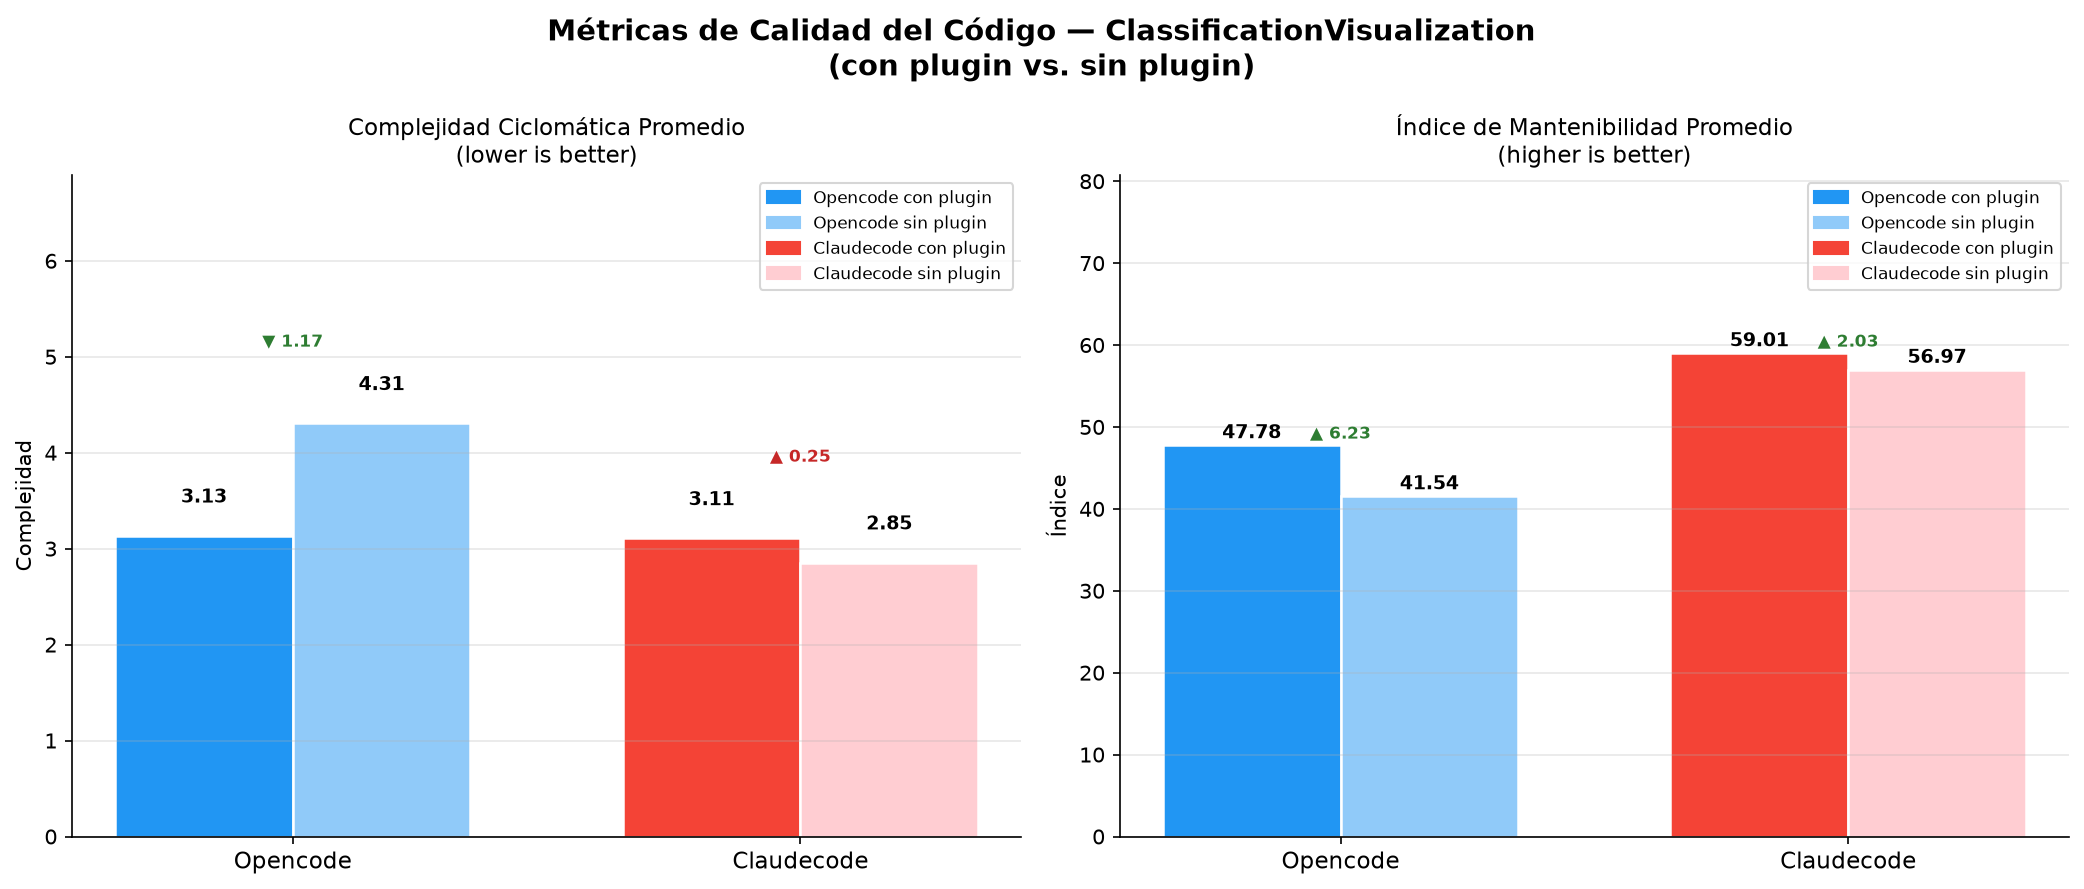
\includegraphics[width=0.90\linewidth, keepaspectratio]{graficos/01_calidad_codigo.png}
        \caption{Métricas de calidad del código (con plugin vs.\ sin plugin)}
    \end{figure}
\end{frame}

% ============================================================
% SLIDE 23: CALIDAD -- EFECTO DEL PLUGIN
% ============================================================
\begin{frame}{Calidad -- efecto del plugin}
    \begin{figure}
        \centering
        
\includegraphics[width=0.90\linewidth, keepaspectratio]{graficos/comparisons/08_delta_calidad.png}
        \caption{Efecto del plugin (delta = plugin $-$ baseline)}
    \end{figure}
\end{frame}

% ============================================================
% SLIDE 24: CASO 1 – CON Y SIN PLUGIN
% ============================================================
\begin{frame}{Caso 1 -- Con y sin plugin}
    \begin{columns}[T]
        \begin{column}{0.49\textwidth}
            \begin{figure}
                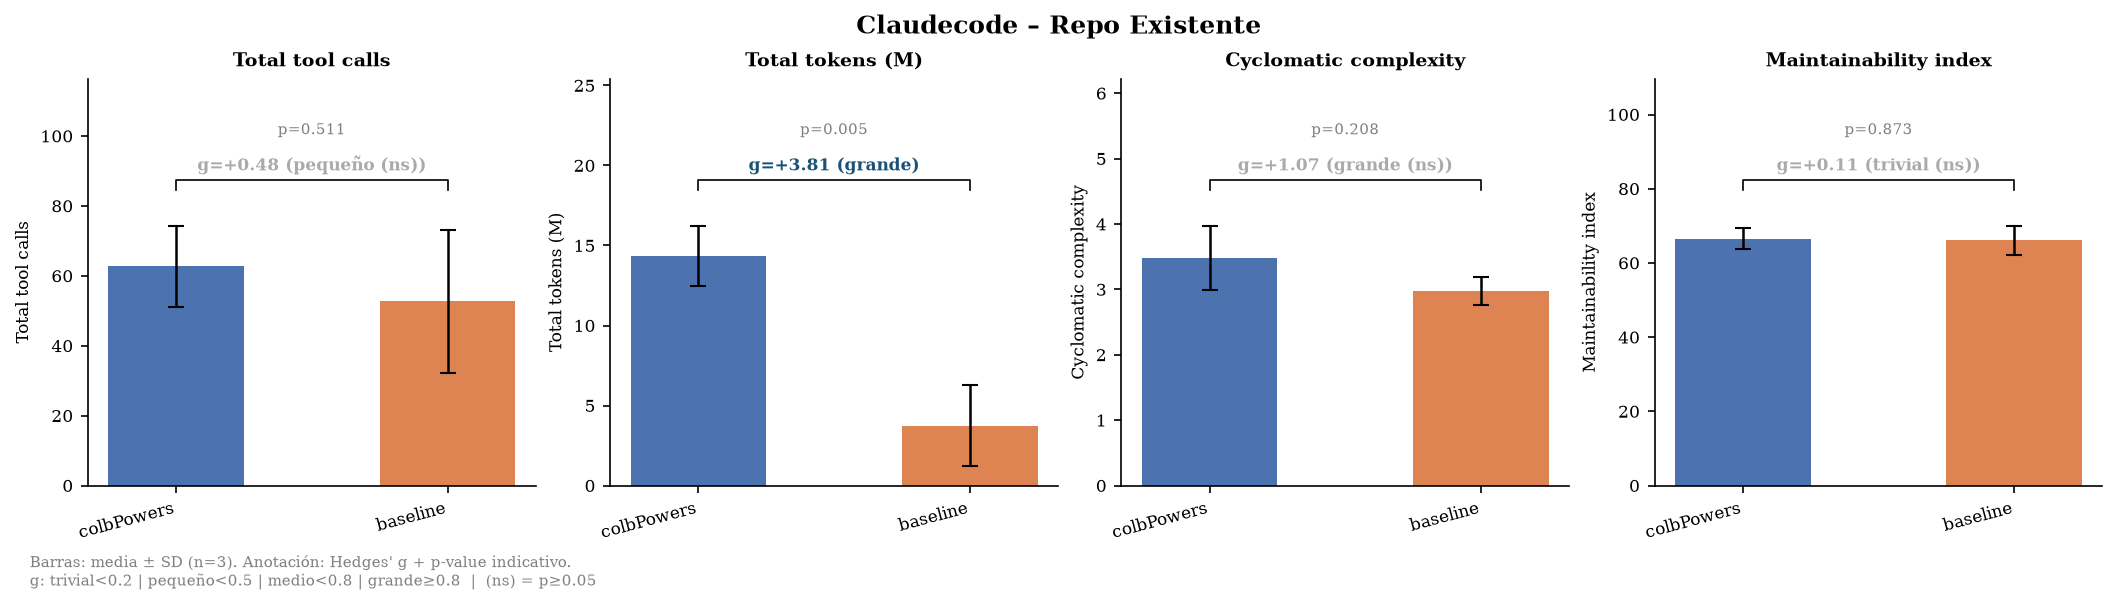
\includegraphics[width=\linewidth, keepaspectratio]{graficos/ttest_analisis/results_cpbl_bars_Claudecode_-_Repo_Existente.png}
                \caption{Claudecode -- Repo Existente}
            \end{figure}
        \end{column}
        \begin{column}{0.49\textwidth}
            \begin{figure}
                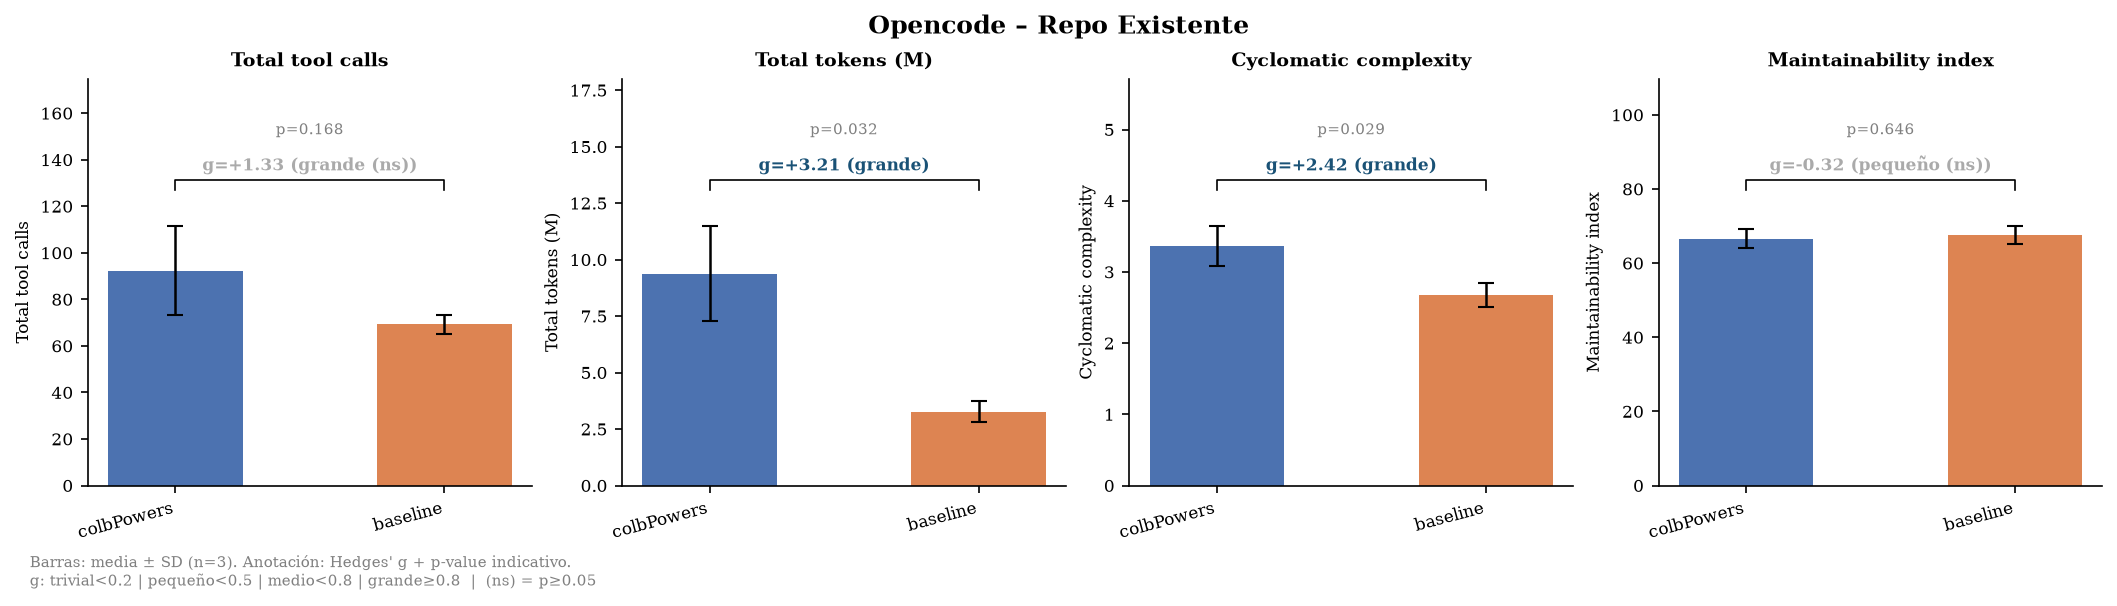
\includegraphics[width=\linewidth, keepaspectratio]{graficos/ttest_analisis/results_cpbl_bars_Opencode_-_Repo_Existente.png}
                \caption{Opencode -- Repo Existente}
            \end{figure}
        \end{column}
    \end{columns}
\end{frame}

% ============================================================
% SLIDE 25: CASO 1 – OPENCODE VS CLAUDECODE
% ============================================================
\begin{frame}{Caso 1 -- Opencode vs.\ Claudecode}
    \begin{columns}[T]
        \begin{column}{0.49\textwidth}
            \begin{figure}
                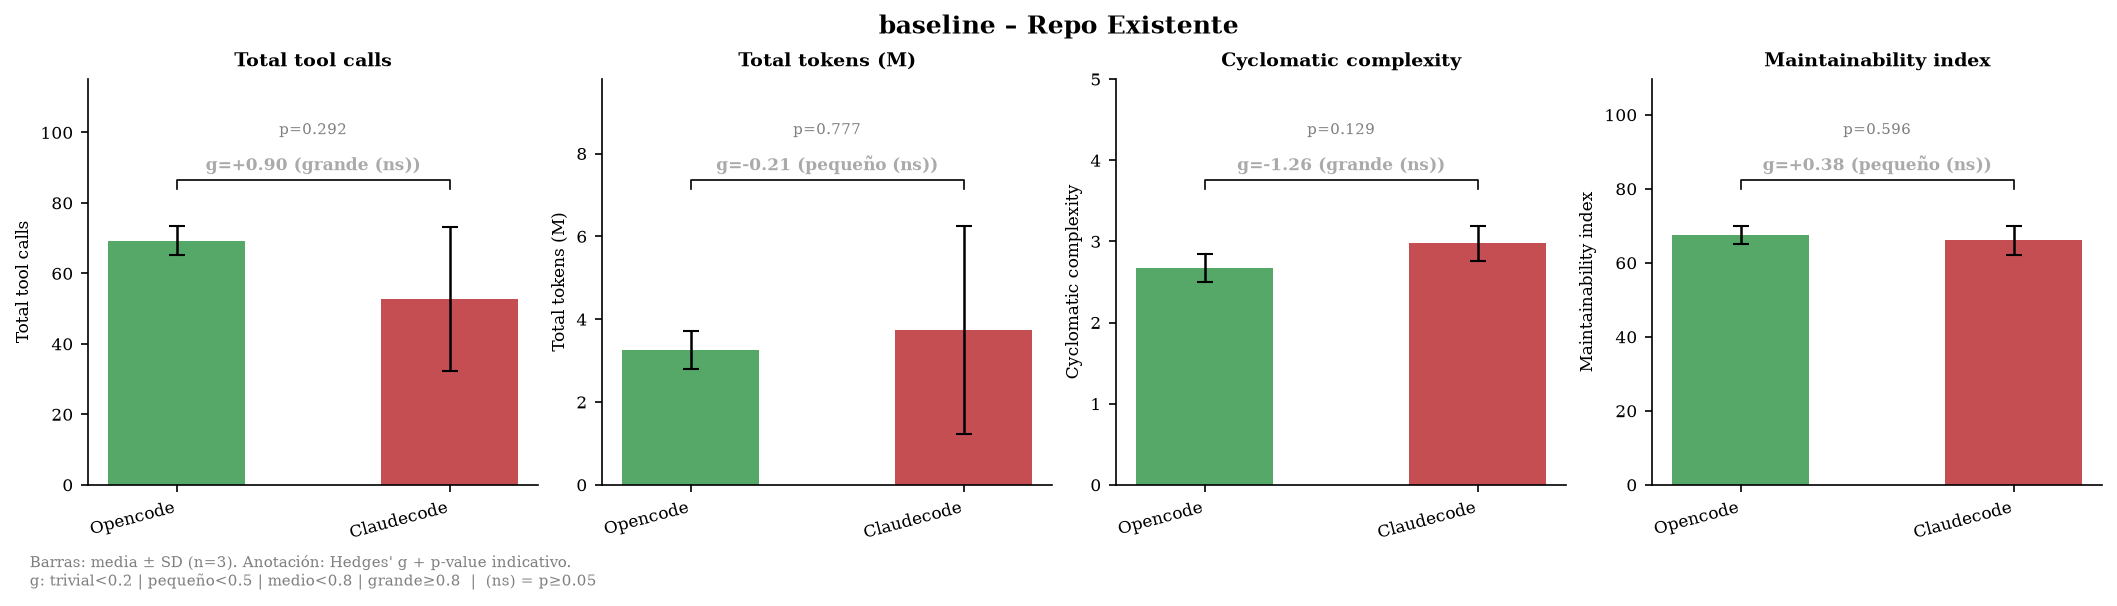
\includegraphics[width=\linewidth, keepaspectratio]{graficos/ttest_analisis/results_occc_bars_baseline_-_Repo_Existente.png}
                \caption{Baseline -- Repo Existente}
            \end{figure}
        \end{column}
        \begin{column}{0.49\textwidth}
            \begin{figure}
                
\includegraphics[width=\linewidth, keepaspectratio]{graficos/ttest_analisis/results_occc_bars_colbPowers_-_Repo_Existente.png}
                \caption{colbPowers -- Repo Existente}
            \end{figure}
        \end{column}
    \end{columns}
\end{frame}

% ============================================================
% SLIDE 26: CASO 2 – CON Y SIN PLUGIN
% ============================================================
\begin{frame}{Caso 2 -- Con y sin plugin}
    \begin{columns}[T]
        \begin{column}{0.49\textwidth}
            \begin{figure}
                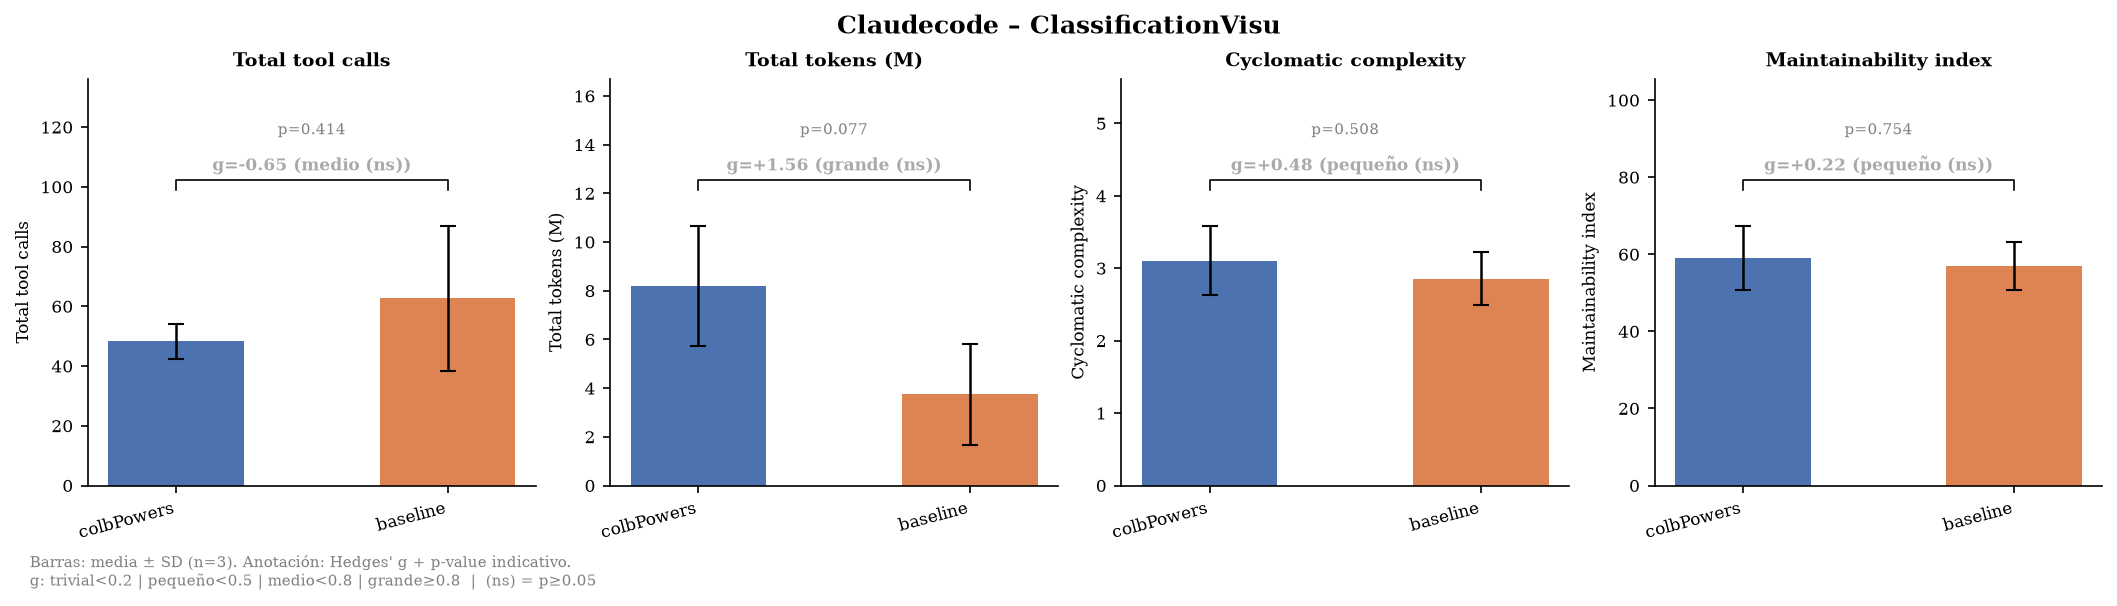
\includegraphics[width=\linewidth, keepaspectratio]{graficos/ttest_analisis/results_cpbl_bars_Claudecode_-_ClassificationVisu.png}
                \caption{Claudecode -- ClassificationVisu}
            \end{figure}
        \end{column}
        \begin{column}{0.49\textwidth}
            \begin{figure}
                
\includegraphics[width=\linewidth, keepaspectratio]{graficos/ttest_analisis/results_cpbl_bars_Opencode_-_ClassificationVisu.png}
                \caption{Opencode -- ClassificationVisu}
            \end{figure}
        \end{column}
    \end{columns}
\end{frame}

% ============================================================
% SLIDE 27: CASO 2 – OPENCODE VS CLAUDECODE
% ============================================================
\begin{frame}{Caso 2 -- Opencode vs.\ Claudecode}
    \begin{columns}[T]
        \begin{column}{0.49\textwidth}
            \begin{figure}
                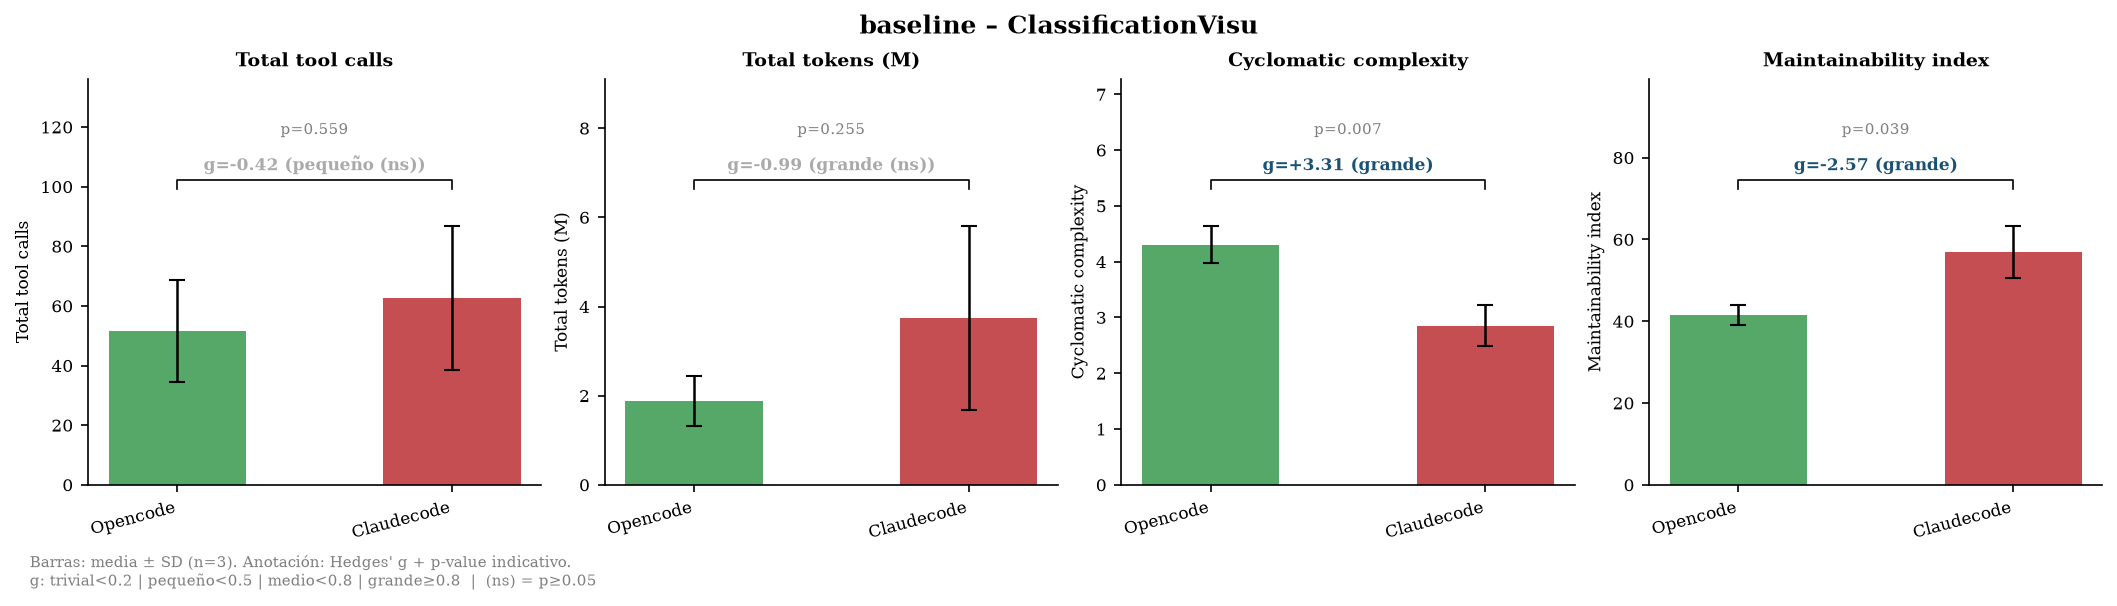
\includegraphics[width=\linewidth, keepaspectratio]{graficos/ttest_analisis/results_occc_bars_baseline_-_ClassificationVisu.png}
                \caption{Baseline -- ClassificationVisu}
            \end{figure}
        \end{column}
        \begin{column}{0.49\textwidth}
            \begin{figure}
                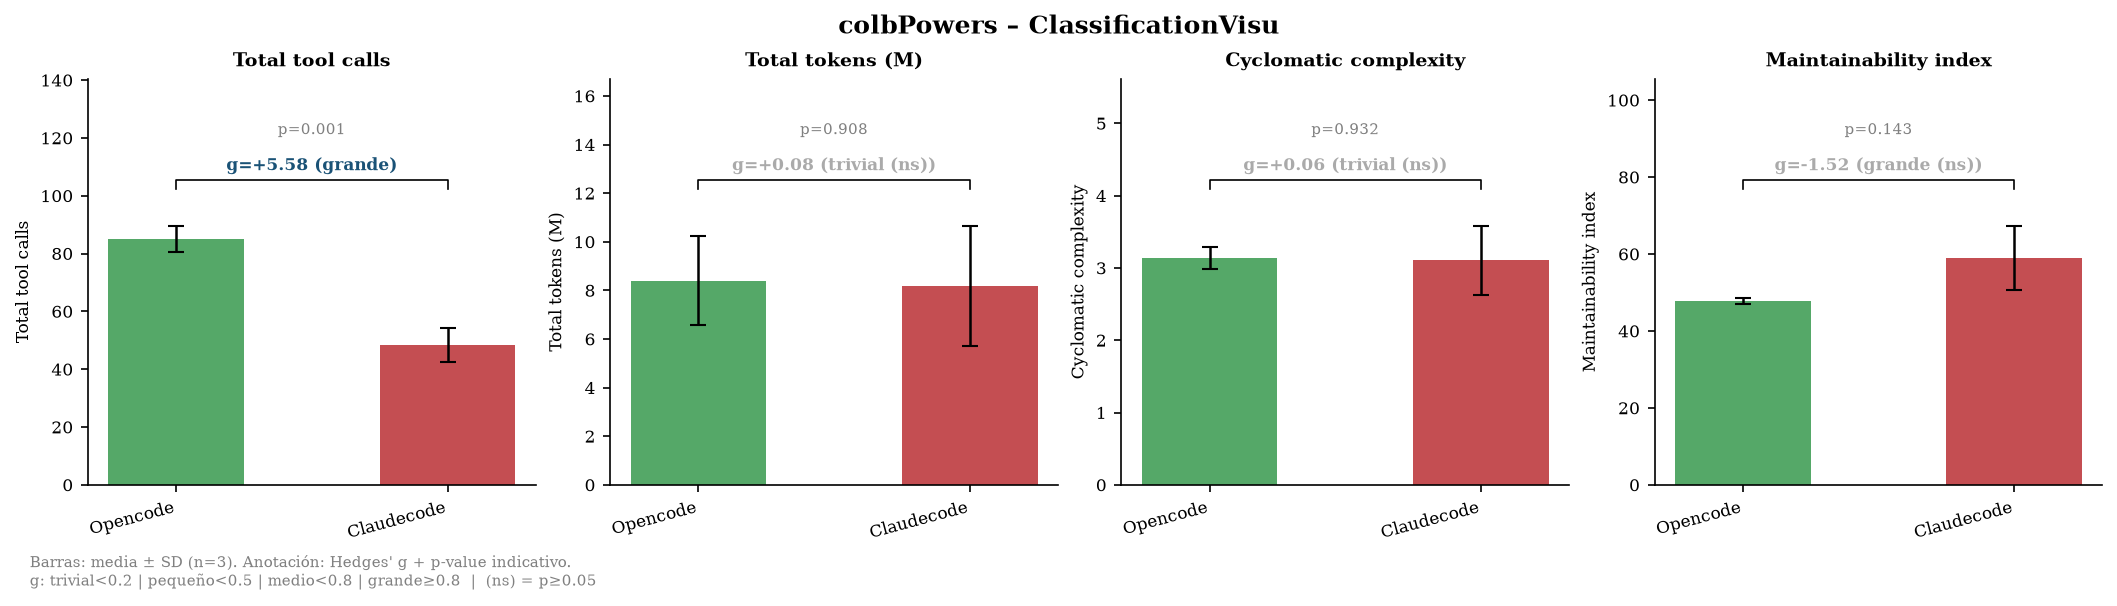
\includegraphics[width=\linewidth, keepaspectratio]{graficos/ttest_analisis/results_occc_bars_colbPowers_-_ClassificationVisu.png}
                \caption{colbPowers -- ClassificationVisu}
            \end{figure}
        \end{column}
    \end{columns}
\end{frame}

% ============================================================
% SLIDE 28: SECTION DIVIDER – CONCLUSIONES
% ============================================================
\begin{frame}[plain,noframenumbering]
\begin{tikzpicture}[remember picture, overlay]
    \fill[MyBlue] (current page.south west) rectangle (current page.north east);
\end{tikzpicture}
\vspace{0.38\textheight}
\begin{center}
    \textcolor{white}{\LARGE Conclusiones}
\end{center}
\end{frame}

% ============================================================
% SLIDE 29: CONCLUSIONES
% ============================================================
\begin{frame}{Conclusiones}
    \begin{itemize}
        \item \textbf{colbPowers} mejora la calidad del código generado en la mayoría de configuraciones evaluadas.
        \vspace{0.2cm}
        \item El efecto es más consistente y significativo con \textbf{Opencode}, especialmente en proyectos nuevos (Caso 2).
        \vspace{0.2cm}
        \item El uso del plugin incrementa el consumo de tokens, pero la relación calidad/coste resulta favorable.
        \vspace{0.2cm}
        \item La metodología \textbf{human-in-the-loop} con documentación estructurada (\texttt{constitution.md} + \texttt{features.md}) es viable y reproducible en entornos reales.
    \end{itemize}
\end{frame}

% ============================================================
% FINAL PAGE
% ============================================================
\begin{frame}[c]
    \centering
    \vfill
    \Huge {Gracias por vuestra atención}
    \Large {¿Preguntas?}
    \vspace{1cm}
    \vfil
\end{frame}

\end{document}
